% !TEX root = ./diss.tex

\chapter{Experiment 1}

This experiment provides an investigation into how neural activity during paired associate learning changes as a function of massed or spaced practice.
% and how it is further modulated by subsequent memory performance

\section{Method}

\subsection{Participants}

% 1-7 were technically pilots

% subNum = [1,2,3,4,5,6,7,8,9,10,11,12,13,14,15,16,17,18,19,20,21,22,27,29,37,39,23,24,25,26,28,30,32,34,47,49,36];
% age = [18,20,18,20,18,20,18,23,19,23,20,20,22,20,19,23,22,20,22,19,18,21,18,19,26,18,26,26,19,19,19,18,19,21,25,20,21];
% gender = [1,1,1,1,1,1,2,1,2,1,2,1,1,2,1,1,1,2,2,2,2,1,1,1,1,1,1,1,2,1,2,2,1,1,2,1,2]; % (1 = male, 2 = female)
% %excludedSub = [1,8,17,19,30];
% %excludedSub = [1,8,17,19,30,5,9,14,15,18,25,28,32,36];
% excludedSub = [];
% numSub = sum(~ismember(subNum,excludedSub))
% mean(age(~ismember(subNum,excludedSub)))
% min(age(~ismember(subNum,excludedSub)))
% max(age(~ismember(subNum,excludedSub)))
% sum(gender(~ismember(subNum,excludedSub)) == 2) % females

Thirty-seven University of Colorado Boulder undergraduates participated in the experiment for either course credit ($n=17$) or payment of \$15 per hour ($n=20$) (ages 18--26, $M=20.5$; 13 female).  All participants were right-handed native-English speakers and had normal or corrected-to-normal vision.  Informed consent was obtained from each participant, and the study conformed to the
% Human Research Committee
Institutional Review Board guidelines.

\subsection{Materials}

The experimental stimuli were randomly selected from 1521 common nouns (the PEERS word pool\footnote{http://memory.psych.upenn.edu})
%\footnote{from the Computational Memory Laboratory at the University of Pennsylvania}
and 832 images (two categories: 371 face images and 461 living room scenes).  Face images were shoulder-up photographs taken in front of an off-white background with the center of the face generally in the center of the image \cite{PhilEtal2000}.  Scene images were photographs taken from the SUN image database within the ``Living Room'' category \cite{XiaoEtal2010}.  Words were presented in Courier font (size 24) and all images were cropped to be the same size ($480\times320$ pixels).  Stimuli were presented on a 17-in flat-panel display with a resolution of $1024\times768$ (60 Hz frame rate) placed 1~m in front of the participants.  All portions of the display not occupied by stimuli or text were filled with gray pixels.

The experiment was programmed in MATLAB (versions R2012b and R2014a; The MathWorks, Inc., Natick, MA) using our experimental framework\footnote{https://github.com/warmlogic/expertTrain} and was presented using Psychtoolbox \cite{Brai1997}.

\subsection{Design}

Experiment~1 consisted of six blocks of four experimental phases (Figure~\ref{fig:space_exp}): exposure, study, distractor, test.  The session, including application of the electrode net and running in the task, lasted approximately 2.5 hours.  Stimuli were randomly shuffled prior to creating the list for each phase at the beginning of the session.  The study phase contained the conditions that were manipulated within subjects, namely the viewing of spaced and massed paired associates.

\subsection{Procedure}

An electrode net was applied to each participant's head, and the session began with a shortened practice version of the experiment to familiarize participants with the study and test procedures (two spaced, two massed, and two single presentation items, with a lag of 4 items between spaced presentations; two new images were included at test).

% \begin{figure}
%   \centering
%   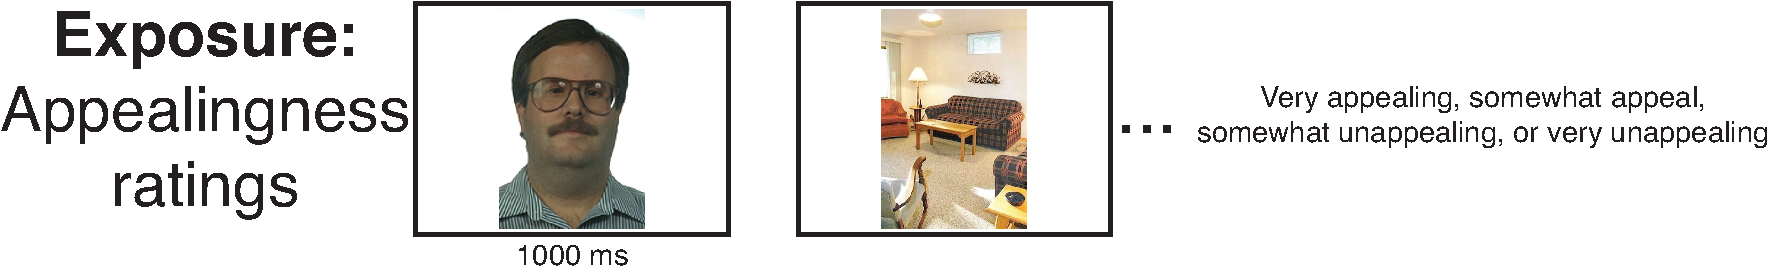
\includegraphics[width=\textwidth]{./figs/exp1/space_example_expo}
%   \caption{Experiment~1: Exposure phase}
%   \label{fig:space_expo}
%   %\ref{fig:space_expo}
%   %\pageref{fig:space_expo}
% \end{figure}

\begin{figure}
  \centering
  \begin{tabular}{l}
  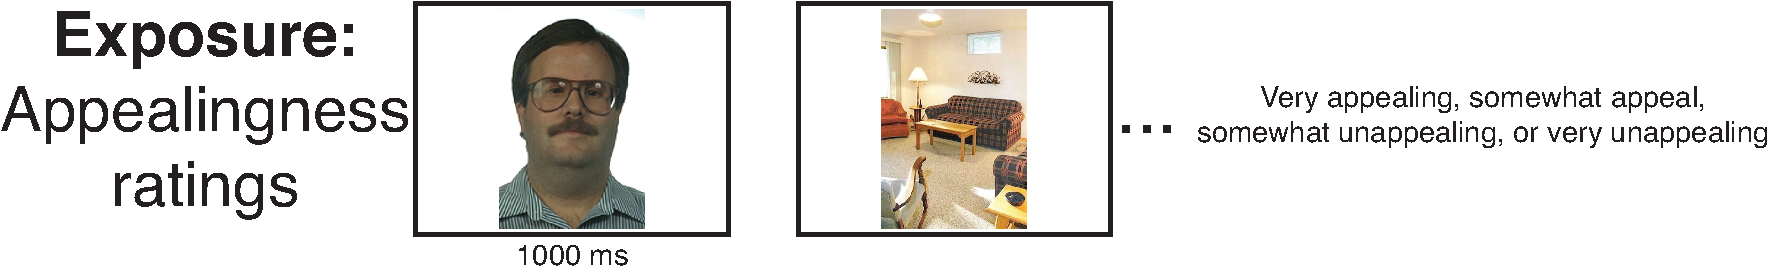
\includegraphics[width=.8\textwidth]{./figs/exp1/space_example_expo} \\
  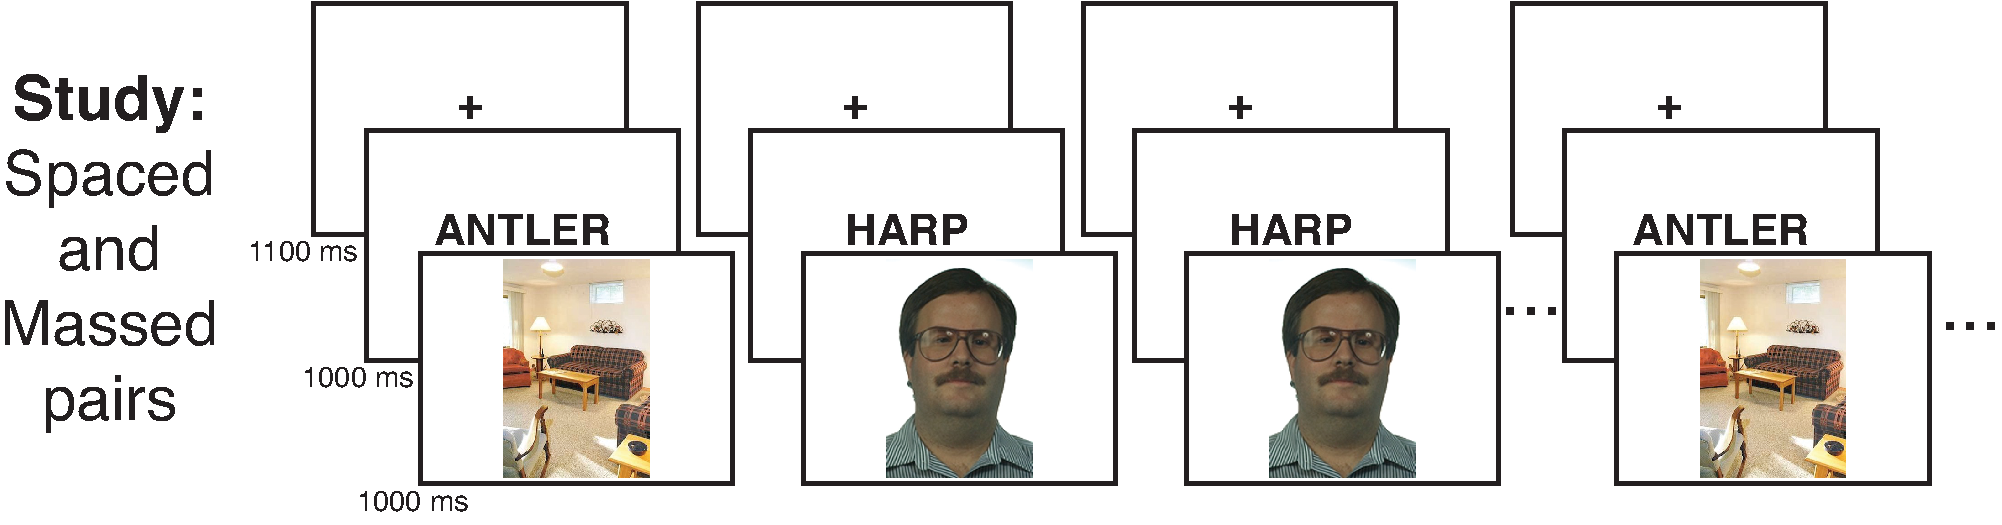
\includegraphics[width=.9\textwidth]{./figs/exp1/space_example_study_fix} \\
  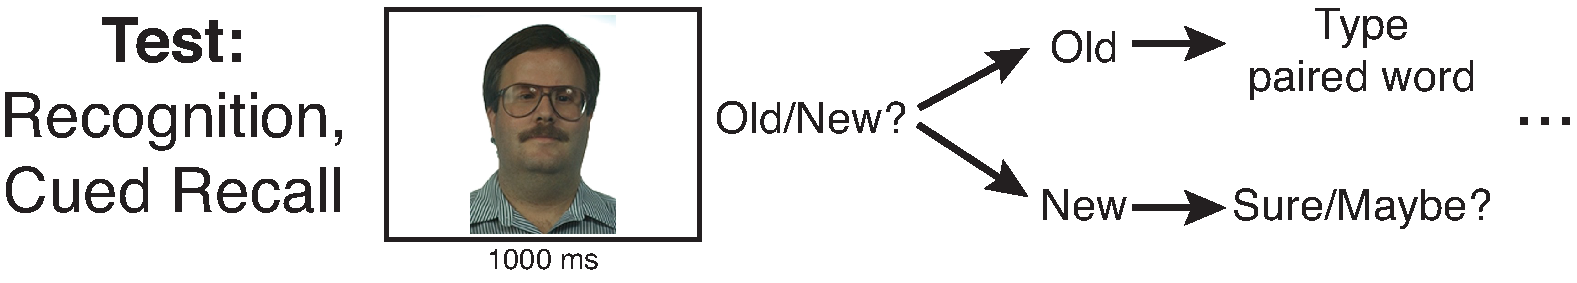
\includegraphics[width=.7\textwidth]{./figs/exp1/space_example_test}
  \end{tabular}
  \caption{Experiment~1: Exposure, study, and test phases}
  \label{fig:space_exp}
  %\ref{fig:space_exp}
  %\pageref{fig:space_exp}
\end{figure}

In the exposure phase, participants viewed the 50 images (half faces and half scenes, randomly intermixed) that they would subsequently see on the study list and rated each on a four-point ``appealing'' scale: very appealing, somewhat appealing, somewhat unappealing, and very unappealing.  Only the images from the upcoming study period were presented; the words were not shown.  The keys {\tt D}, {\tt F}, {\tt J}, and {\tt K} were used to make the response, and the scale-to-keyboard mapping was counterbalanced across participants.  An image denoting the key--response mapping was shown at the bottom of the screen at all times, but participants were encouraged to memorize the keys so they could keep their eyes on the fixation cross at the center of the screen.  On each trial, a cross was shown for 1.0--1.2~s (jittered), then the cross and image were shown for 1.0~s, after which the cross changed to a question mark prompting participants to make a response.  Participants were allowed to respond during the initial 1.0~s image presentation; if this occurred, the image stayed on screen for a total of 1.0~s.  If they waited longer than 1.0~s and the cross changed to a question mark, the image remained on screen until a response was made or 3.0~s passed.  No more than three images from the same category could occur in a row. This phase lasted approximately 3~min.

% The face and house presentations can be used for training classifiers.  \hl{(out of context, should explain what I mean by classifiers.)}

% 3.0~s timer for exposure response

% \begin{figure}
%   \centering
%   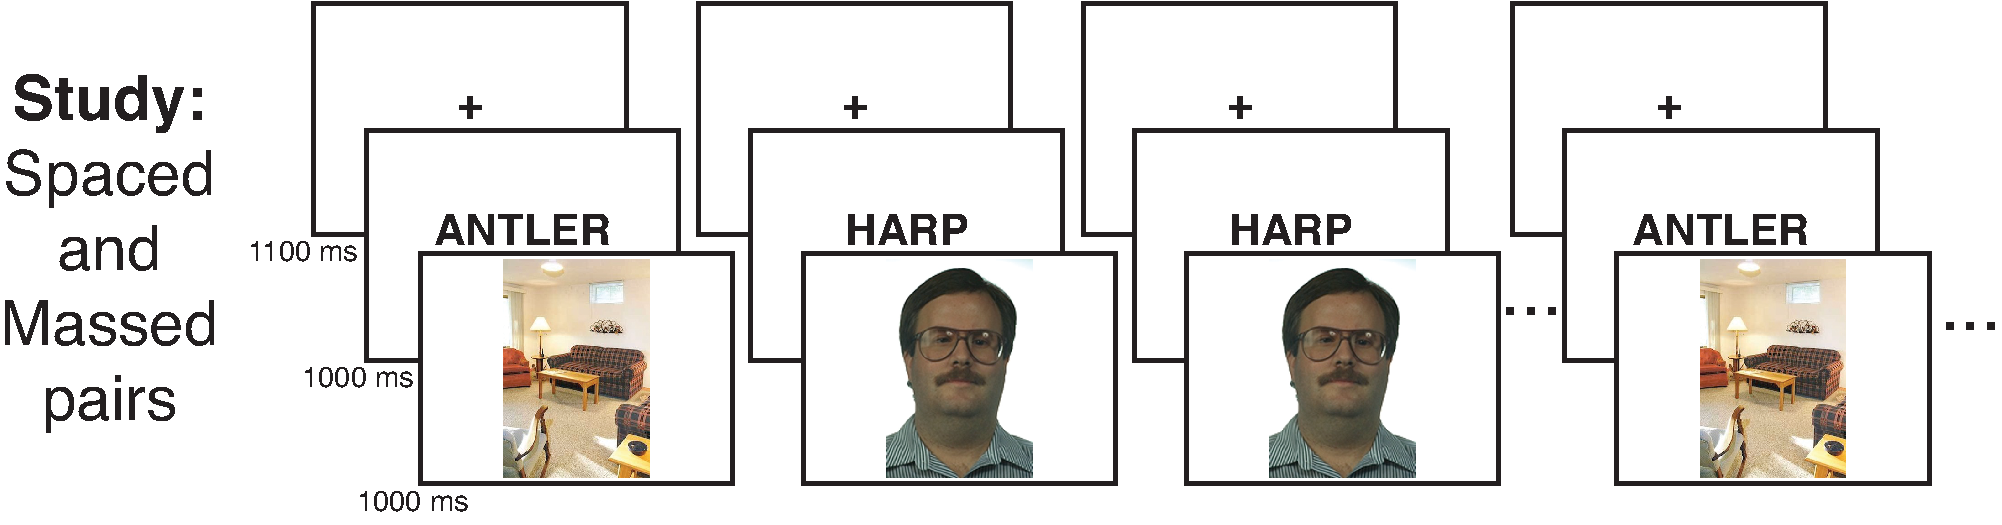
\includegraphics[width=.9\textwidth]{./figs/exp1/space_example_study_fix}
%   \caption{Experiment~1: Study phase}
%   \label{fig:space_study}
%   %\ref{fig:space_study}
%   %\pageref{fig:space_study}
% \end{figure}

In the study phase, participants viewed 50 word--image pairs and were asked to think of a relationship between them or to make up a story pairing them.  They were told that a subsequent test would require them to remember the word associated with each picture, but they were not told that some pairs are repeated.  For each of the two image categories there were seven two-presentation spaced pairs, seven two-presentation massed pairs, seven pairs presented only once, and four additional single-presentation buffers (two at the beginning of the list and two at the end).  Only images from the spaced and massed pairs were included on the test list.
% The seven single-presentation items were not tested to keep the experiment from running too long.
Spaced items were presented at a lag of 12 (12 intervening pairs between presentations 1 and 2), and massed items were presented at a lag of zero.  On each trial, a fixation cross appeared for 1.0--1.2~s (jittered), then the word was presented first for 1.0~s followed immediately by the image for 1.0~s.  No more than three images from the same category could occur in a row, and no more than two trials with the same lag (including single-presentation pairs) could occur in a row.  Each study phase lasted approximately 5~min.

In the distractor phase, participants answered simple math problems of the format \texttt{A+B+C=?} for either 2~min or until they answered 60 problems, whichever came first.  They typed their responses with the keyboard. Different tones occurred for correct and incorrect answers, and mean accuracy and response time was reported to the participant at the end of the phase.

% \begin{figure}
%   \centering
%   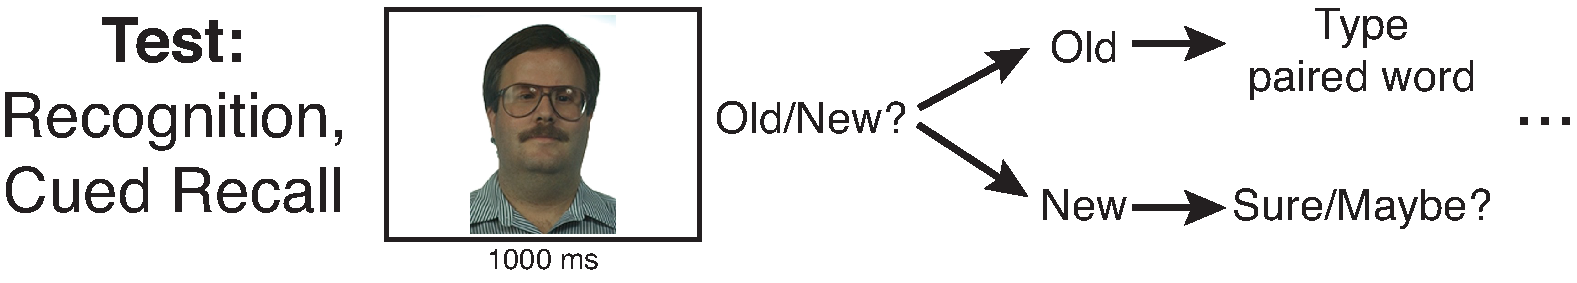
\includegraphics[width=\textwidth]{./figs/exp1/space_example_test}
%   \caption{Experiment~1: Test phase}
%   \label{fig:space_test}
%   %\ref{fig:space_test}
%   %\pageref{fig:space_test}
% \end{figure}

Finally, in the test phase, participants performed recognition and cued recall tasks.  Twenty-eight old images (seven spaced and seven massed from each category) and 14 new images (seven lures from each category) were mixed together and presented one at a time, at which point participants made two responses.  First, they had to decide whether the image was studied earlier (``old'') or had not been seen before (``new'') using the \texttt{F} and \texttt{J} keys (counterbalanced).  If they answered ``old'', they saw \texttt{???????} below the image and had to type the word previously paired with the image; they could pass if they could not remember the word.  If they answered ``new'', they either said that they were ``sure'' it was new or it was ``maybe'' new using the \texttt{F} and \texttt{J} keys (counterbalanced); this confidence judgment was used so the same number of responses occurred for both ``old'' and ``new'' items. An image showing the key--response mapping was shown at the bottom of the screen when appropriate, but participants were encouraged to memorize the keys so they could keep their eyes fixated on the cross.  On each trial, a fixation cross appeared for 1.0--1.2~s (jittered) and the image was shown for 1.0~s, at which point the cross turned to a question mark and participants were asked to make their initial recognition response.  With lures mixed in, no more than four images from the same category could occur in a row.  Importantly, test images were presented in a sequence similar to the study order.  To construct the test list, the positions of the second presentations of study stimuli were divided into five contiguous groups and each group was randomly shuffled.  This was done to approximately preserve a similar amount of time between the second presentation and the test across all ``old'' stimuli.  Each test phase lasted approximately 4 to 5~min.

% 3.0~s timer for recognition and new responses

% There were approximately 7~min between studying a spaced or massed word--image pair and seeing that image on the test list.

\subsection{Electrophysiological recordings and data processing}

\begin{figure}
  \centering
  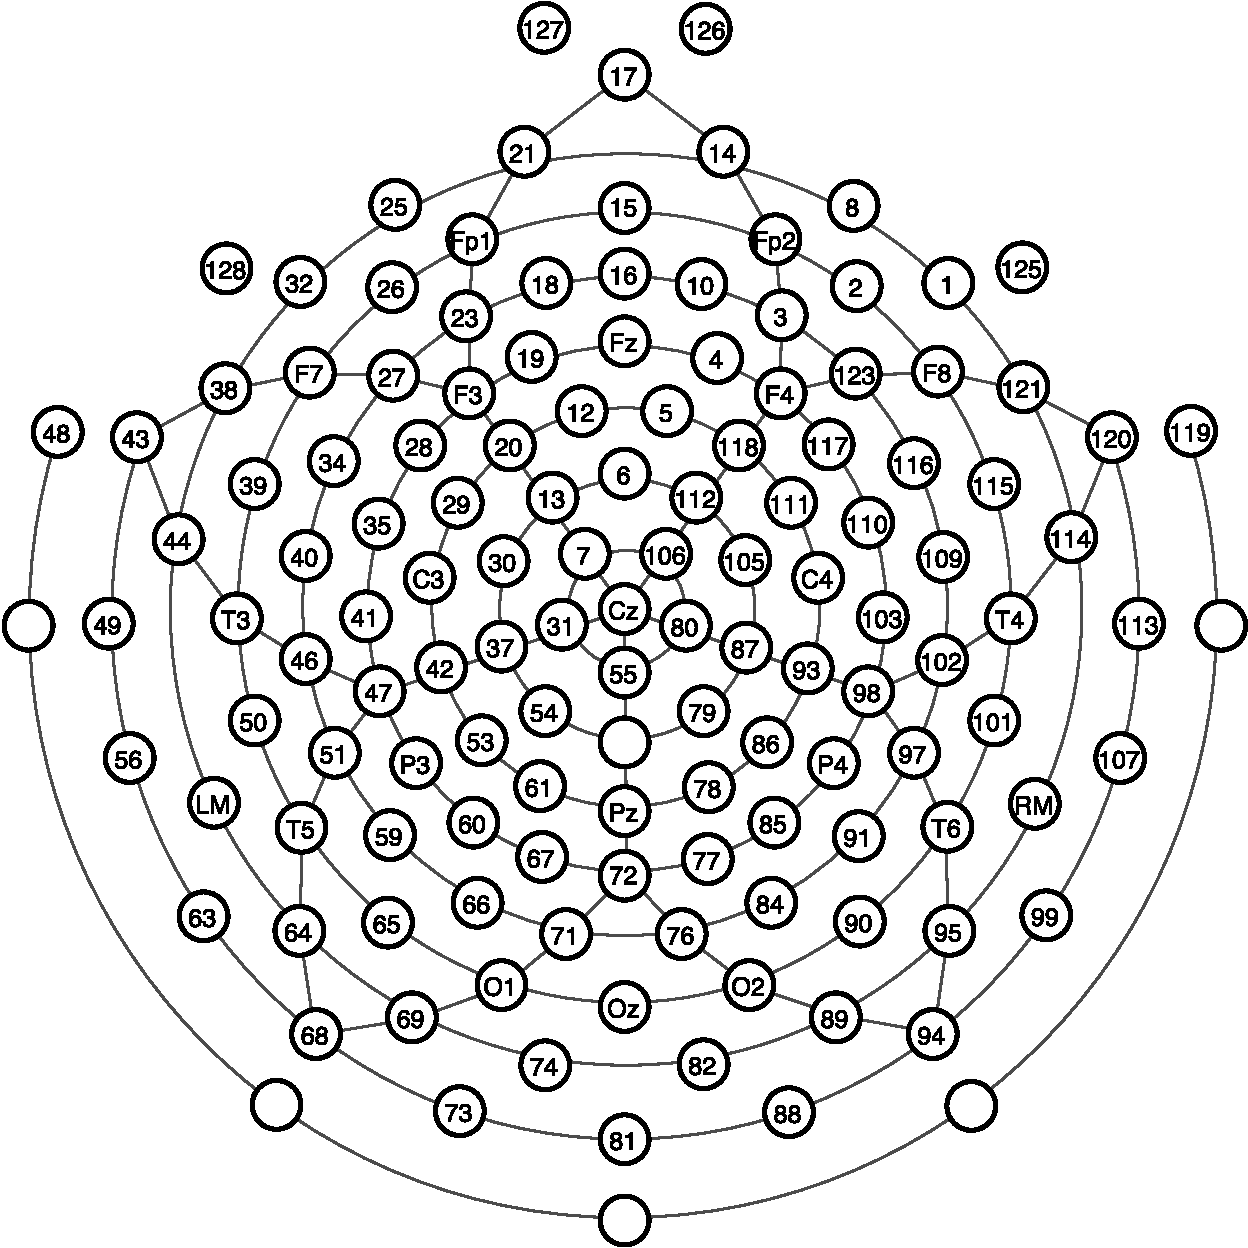
\includegraphics[width=.40\textwidth]{./figs/hcgsn_full}
  \caption{The 128-channel HydroCel Geodesic Sensor
    Net\texttrademark{} used to measure the EEG.  In this top-down schematic the participant's nose is toward the front.}
  \label{fig:roi}
  %Figure~\ref{fig:roi}
\end{figure}

A 128-channel HydroCel Geodesic Sensor Net\texttrademark{} (GSN~200, v.~$2.1$; \citeNP{Tuck1993}) was used to measure the EEG at the scalp using a central vertex reference (Cz) with a sampling rate of $250$~Hz and a low-pass hardware filter at $100$~Hz (see Figure~\ref{fig:roi}).  The net was connected to an AC-coupled, high-input impedance amplifier ($300$~M$\Omega$, Net~Amps\texttrademark{}; Electrical Geodesics, Inc., Eugene, OR) and recordings were made using the Net Station application.  The electrodes were adjusted until impedance measurements were less than $40$~k$\Omega$.

All data processing steps and analyses were done in MATLAB using in-house scripts\footnote{https://github.com/warmlogic/mat-mvm} and the FieldTrip toolbox \cite{OostEtal2011}.  A high-pass filter at $0.1$~Hz, low-pass filter at $100$~Hz, and a notch filter from $59$--$61$~Hz were applied to the data.  Study and test trials were epoched into $3000$~ms segments, $1$~s before the onset of each stimulus and $2$~s after.  Artifact detection was used to reject particularly noisy epochs, as well as those that exceed an amplitude of $\pm100~\mu$V.  The data were referenced to the average of all channels and individual trials were baseline corrected relative to -$200$~ms to $0$~ms.

% Independent components analysis (ICA) was used to remove blink artifacts and other consistent noise, and artifact detection was run again with more stringent settings to reject noisy trials.

We would not expect differences in neural activity between the initial presentations of spaced and massed items, as the locus of the spacing effect occurs after this point.
% No differences were found [$F$s~$<1.0$].
There may exist subsequent memory effects here, though it would be difficult to know whether neural activity during the first presentation is the reason for this effect (e.g., perhaps a subsequently remembered item was encoded poorly on the first presentation and very well on the second presentation).  ERP analyses included these initial presentations in analyses as a baseline, but time--frequency analyses focused on the second presentation (the repetition) and show the single-presentation stimuli in data plots.
\cbstart
The repetition is therefore the critical trial type to analyze, as this is where the massed and spaced manipulation occurs, and plots will focus on the repetition.  The first presentation is included in the analysis to see whether activity changes differently across presentations for massed and spaced items (the ANOVA factor of presentation).  To foreshadow some results, there were no differences between first presentations of massed and spaced items in ERP analyses; these trials were not included in time--frequency analyses.
\cbend


% control condition
% \hl{Since spacing effect theories implicate differences in these cognitive processes during massed and spaced repetitions, the initial presentations were used as the control condition (presentation number was a factor in our ANOVAs).  There should be no difference between the initial presentations and thus the contrast with this control will reveal the differences that exist due to repetition lag (a repetition effect).  We are therefore asking what is different between spaced and massed repetitions relative to initial episodic encoding.  Over and above this, we can ask how memory processes are different between the repetition.}


% General encoding mechanisms active during spaced and massed repetitions should be similar.


\section{Results}

% SPACE008 did not perform the task properly

% SPACE001, SPACE017, SPACE019, and SPACE030 had extremely low trial counts

% SPACE039 had really noisy EEG; % or had very noisy EEG ($n=1$)

Thirty-one participants were included in behavioral analyses.  Fourteen participants were excluded from ERP and time--frequency analyses because they either did not perform the task properly ($n=1$, completely excluded) or had fewer than 10 artifact-free trials in any of the main trial conditions ($n=13$; four had extremely low trial counts and were also excluded from behavioral analyses),
% \footnote{New preprocessing methods are ongoing to retain more trials for future analyses.},
leaving twenty-three participants in EEG analyses.  Similarity analyses included the twenty-eight participants who had six or more artifact-free pairs of initial presentation--repetition image trials.

All analyses contingent on subsequent memory are split by whether words were recalled or forgotten after the image was correctly recognized as being old.
Significant results are reported, and unreported results can be assumed to not be significant.
When an ANOVA contains a factor with more than two levels, the reported values are adjusted for violations of assumptions of sphericity using the Greenhouse-Geisser procedure \cite{GreeGeis1959} even if the factors did not violate Mauchly's test of sphericity.

\subsection{Behavioral results}

On average, scenes were rated as more appealing compared to faces ($M=2.99$ vs $M=2.01$) [$t(30)=9.13, p=3.6e^{-10}$].  The average response times during the exposure/rating phase was faster for faces (1027~ms) than scenes (1115~ms) [$t(30)=3.62, p=.0011$].
% Because stimuli were presented for 1000~ms, participants had an overall tendency to respond after image offset; this is simply to note that attention is likely paid to the stimulus throughout its presentation, which is relevant to using these trials to train a classifier to discriminate between EEG activity related to faces and scenes.

% During test, recognition discrimination ($d'$) was high, but a spacing effect still occurred: spaced images ($M=3.05, SEM=0.13$) were recognized significantly better than massed images ($M=2.79, SEM=0.13$) [$t(30)=4.74, p=.00005$].  Words from spaced pairs were recalled significantly better than those from massed pairs.

For the test phase, a two-way repeated measures ANOVA was run on image recognition discrimination ($d'$) with factors of spacing and image category.  There was a main effect of spacing [$F(1,30)=17.4, p=.00024, MSE=0.0756$] such that spaced images ($d'=2.95$) were recognized better than massed images ($d'=2.74$), and a main effect of image category [$F(1,30)=104, p=3.05e^{-11}, MSE=0.224$] such that faces ($d'=3.32$) were recognized better than scenes ($d'=2.37$).  An ANOVA with the same factors was run on cued recall hit rate (for old items called ``old'').  There was only a main effect of spacing [$F(1,30)=81.8, p=4.51e^{-10}$] such that spaced words ($M=49.8\%$) were recalled better than massed words ($M=36.5\%$).  Words paired with faces and scenes were recalled at the same rate (faces: $M=43.7\%$; scenes: $M=42.5\%$).  Thus, there are clear spacing effects for both recognition and recall.

\subsection{ERP results}

ERP analyses were performed on $40$~Hz low-pass filtered data using repeated measures ANOVAs; pairwise comparisons were made with $t$-tests.  Peak electrodes and latencies for the ERP effects were found by collapsing all word presentation events together (using grand averages), finding the electrode with the peak voltage within the effect time ranges, and then locating the peak latency using that electrode and its immediate neighbors.  The peak electrodes had to show typical effect patterns, and ended up being near the electrodes used by \citeA{VanSEtal2007}: Cz for the N400 and a parietal electrode just to the right of Pz (electrode~77) for the LPC effect.  The N400 peaked at $372$~ms (Figure~\ref{fig:N400}).  The LPC peaked at $596$~ms (Figure~\ref{fig:LPC}).  For visual N1, the electrode had to show negative peaks between $150$ and $250$~ms and it should have precedence in the literature.  Electrode~58 (T5) peaked at $172$~ms (Figure~\ref{fig:N1}).  Analyses use these peak electrodes and neighbors; words during the study phase were analyzed because ERPs for images would likely be affected due to immediately following word presentations.

The average voltage and peak latency data used in statistical tests comparing massed and spaced conditions were computed for individual subjects using the electrode locations and time windows described above.  Peak latency was determined by averaging the 10 time samples with the largest voltage, and voltage was averaged across the appropriate sized time window at that peak time point.
Three-way ANOVAs with factors of spacing (spaced and massed), presentation (1/new and 2/old), and subsequent memory (recalled and forgotten words; all trials were subsequent recognition hits) were performed.  Single presentations items were not included because they were not tested, but presentation 1 is a close analogue to a single presentation item for the purpose of comparing our results to the literature.

Since the N400 and LPC have precedent in the repetition literature, we analyzed these components for semantic processing and memory effects, and analyzed the visual N1 for attentional effects.
% We kept the study by \citeA{VanSEtal2007} in mind when choosing electrodes.
%These authors used a multi-electrode factor in their ANOVA but tended to focus on electrode Cz for the N400 and Pz for the LPC.
% \citeA{VanSEtal2007}  analyzed the average of a fixed window (400$\pm$50~ms) for the N400, but used the average of a $\pm$50~ms window centered at each participant's peak amplitude at Pz in LPC analyses.
% We chose data for most analyses by finding the peak electrode and latency for each ERP component, and used a $\pm$50~ms window for the N400 and N1 and a $\pm$100~ms window for the LPC, as late effects tend to spread out more than earlier effects.


% ERP attentional and recognition memory component analyses.

% Again, during studied words the visual N1 peaked at 172~ms (Figure~\ref{fig:N1}), the N400 peaked at 372~ms (Figure~\ref{fig:N400}), and the LPC peaked at 596~ms (Figure~\ref{fig:LPC}).
%The results described below mostly replicate the results of \citeA{VanSEtal2007}; however, no correlations were found between the ERP effects and recall rate.

% This is like the test done by \citeA{VanSEtal2007} but with the added factor of memory.

% Attentional components

% The posterior N2 has been shown to be more negative when paying more attention during a voluntary attention task \cite{FolsVanP2008,SuwaEtal2000}.

% % plot: N1 at E58 + surround and 96 + surround

% \begin{figure}
%   \centering
%   \begin{tabular}{ccc}
%   & Left & Right \\
%   \raisebox{2.2cm}{\rotatebox{90}{Massed}} & 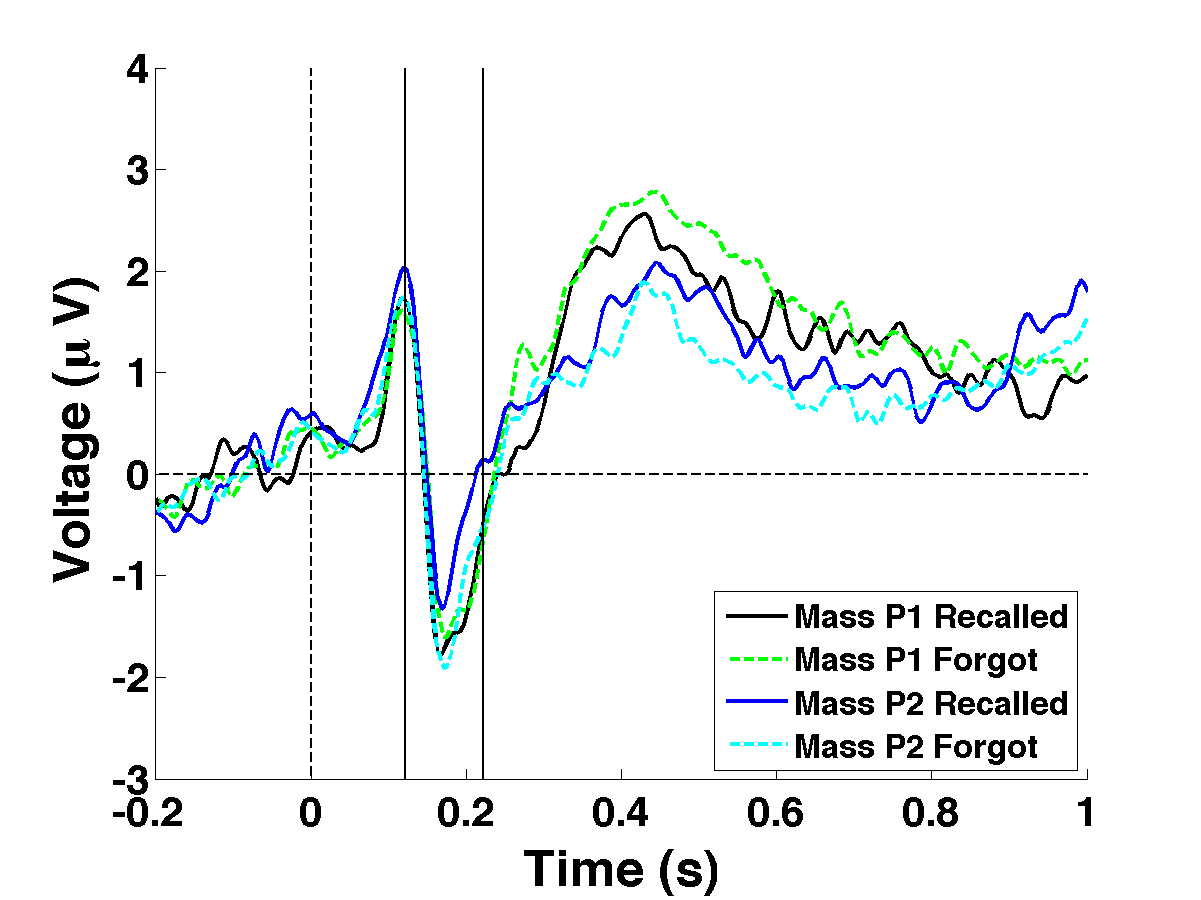
\includegraphics[width=.45\textwidth]{./figs/exp1/tla_single_ga_word_RgH_rc_mass_p1_word_RgH_fo_mass_p1_word_RgH_rc_mass_p2_word_RgH_fo_mass_p2_E50_E51_E57_E58_E59_E64_E65_-200_1000_legend_xylabel} &
%   \includegraphics[width=.45\textwidth]{./figs/exp1/tla_single_ga_word_RgH_rc_mass_p1_word_RgH_fo_mass_p1_word_RgH_rc_mass_p2_word_RgH_fo_mass_p2_E90_E91_E95_E96_E97_E100_E101_-200_1000_legend_xylabel} \\
%   \raisebox{2.2cm}{\rotatebox{90}{Spaced}} & 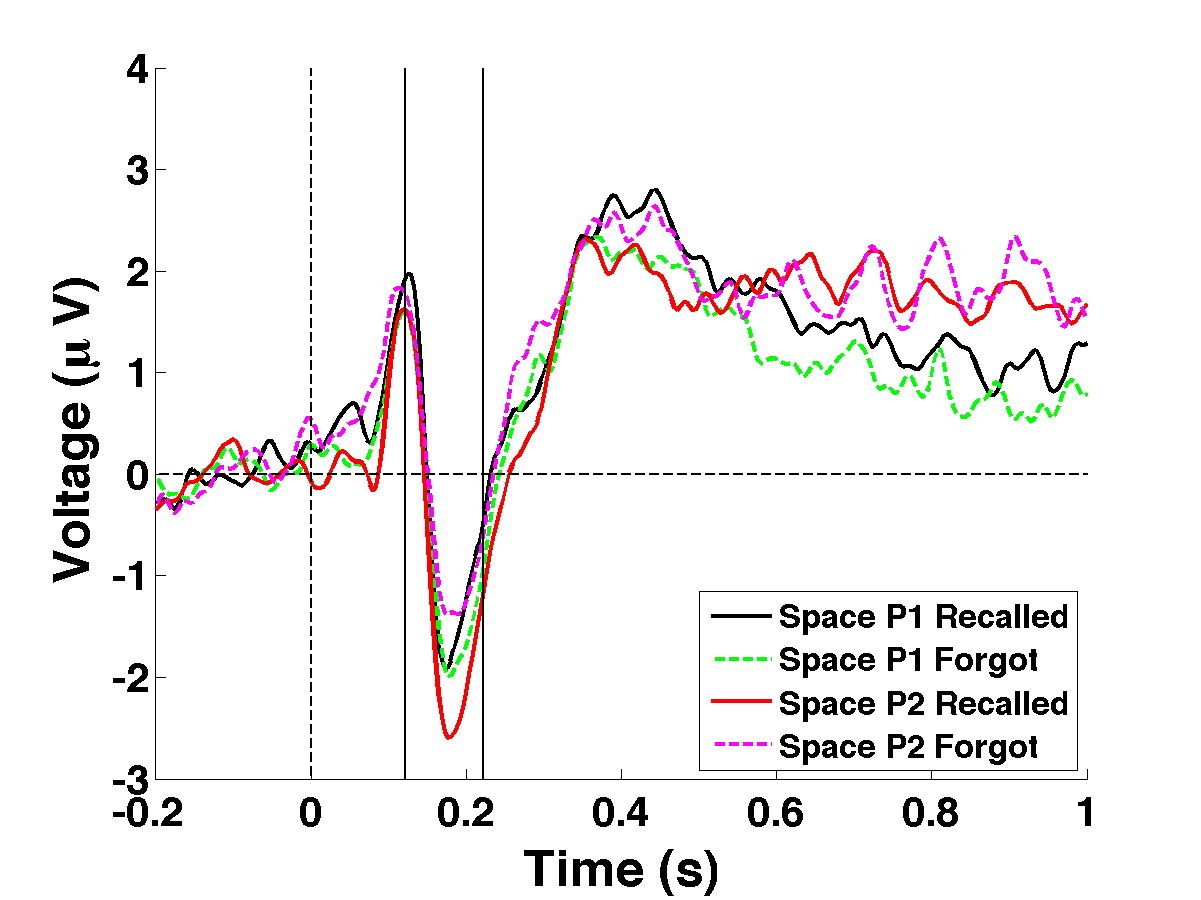
\includegraphics[width=.45\textwidth]{./figs/exp1/tla_single_ga_word_RgH_rc_spac_p1_word_RgH_fo_spac_p1_word_RgH_rc_spac_p2_word_RgH_fo_spac_p2_E50_E51_E57_E58_E59_E64_E65_-200_1000_legend_xylabel} &
%   \includegraphics[width=.45\textwidth]{./figs/exp1/tla_single_ga_word_RgH_rc_spac_p1_word_RgH_fo_spac_p1_word_RgH_rc_spac_p2_word_RgH_fo_spac_p2_E90_E91_E95_E96_E97_E100_E101_-200_1000_legend_xylabel} \\
%   \end{tabular}
%   \caption{N1 to words at electrodes 58 (left) and 96 (right) and neighbors: Massed (top) and spaced (bottom).  The early negative peak is significantly larger for spaced compared to massed repetitions.}
%   \label{fig:N1}
%   %Figure~\ref{fig:N1}
% \end{figure}

% plot: N1 at E58 + surround
\begin{figure}[hp]
  \centering
  \begin{tabular}{cc}
  Massed & Spaced \\
  \multicolumn{1}{l}{(a)} & \multicolumn{1}{l}{(b)} \\
  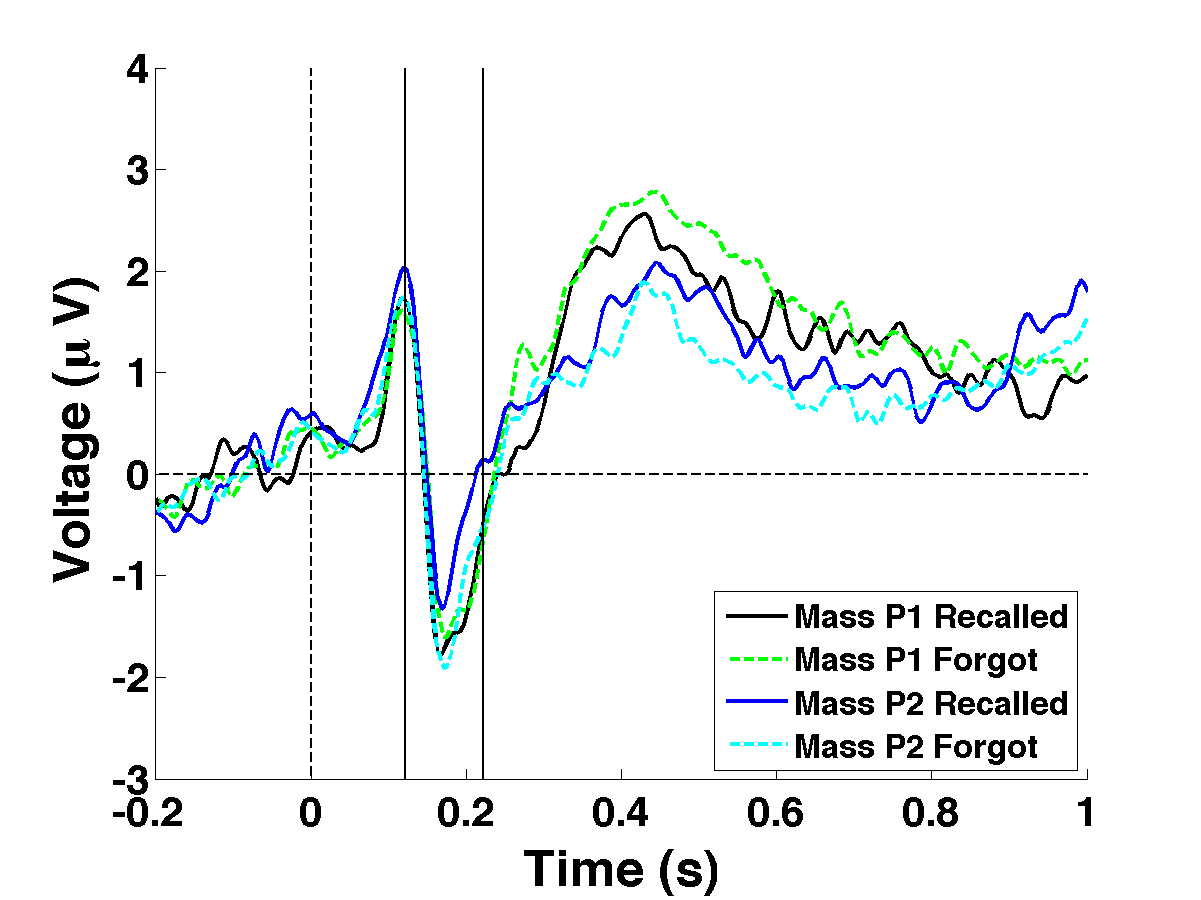
\includegraphics[width=.35\textwidth]{./figs/exp1/tla_single_ga_word_RgH_rc_mass_p1_word_RgH_fo_mass_p1_word_RgH_rc_mass_p2_word_RgH_fo_mass_p2_E50_E51_E57_E58_E59_E64_E65_-200_1000_legend_xylabel} &
  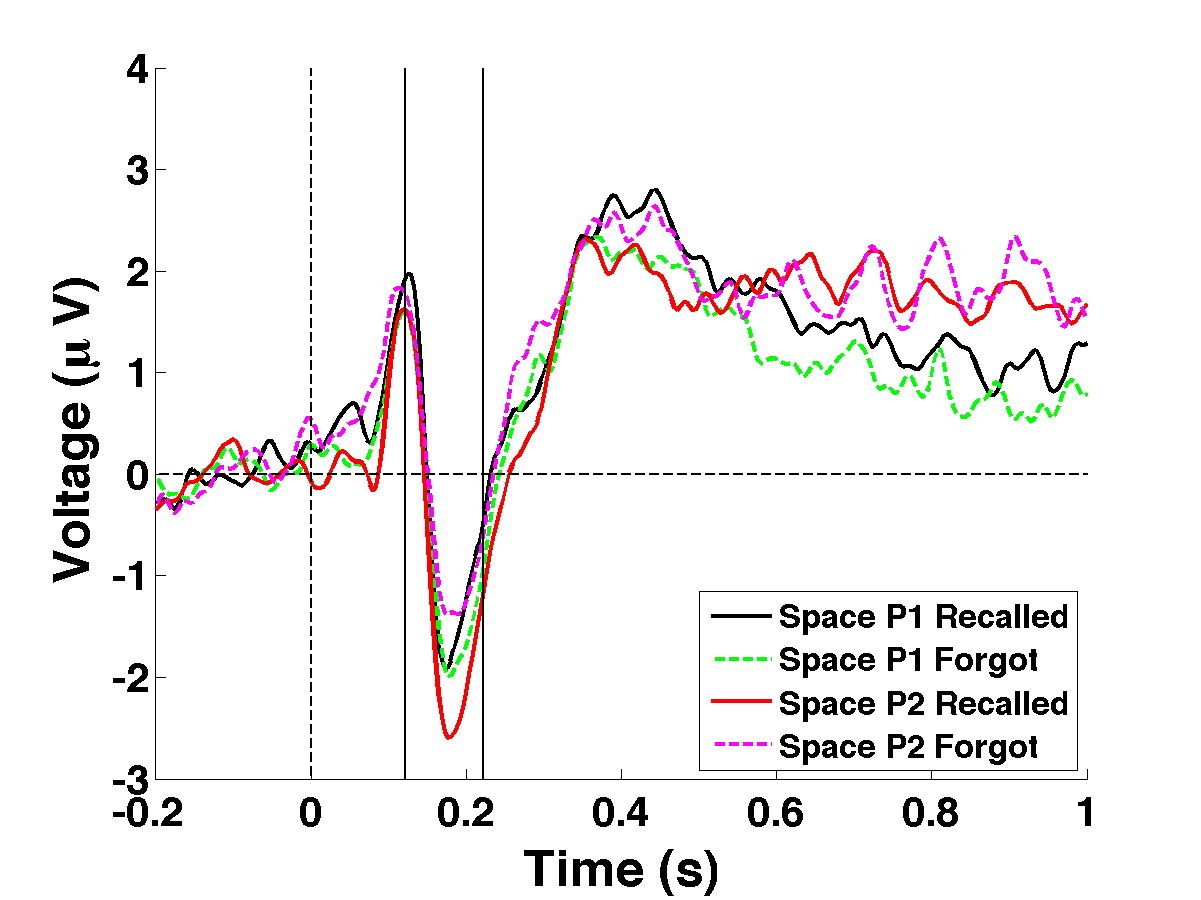
\includegraphics[width=.35\textwidth]{./figs/exp1/tla_single_ga_word_RgH_rc_spac_p1_word_RgH_fo_spac_p1_word_RgH_rc_spac_p2_word_RgH_fo_spac_p2_E50_E51_E57_E58_E59_E64_E65_-200_1000_legend_xylabel} \\
  Recalled P2: Massed $-$ Spaced & Means \\
  \multicolumn{1}{l}{(c)} & \multicolumn{1}{l}{(d)} \\
  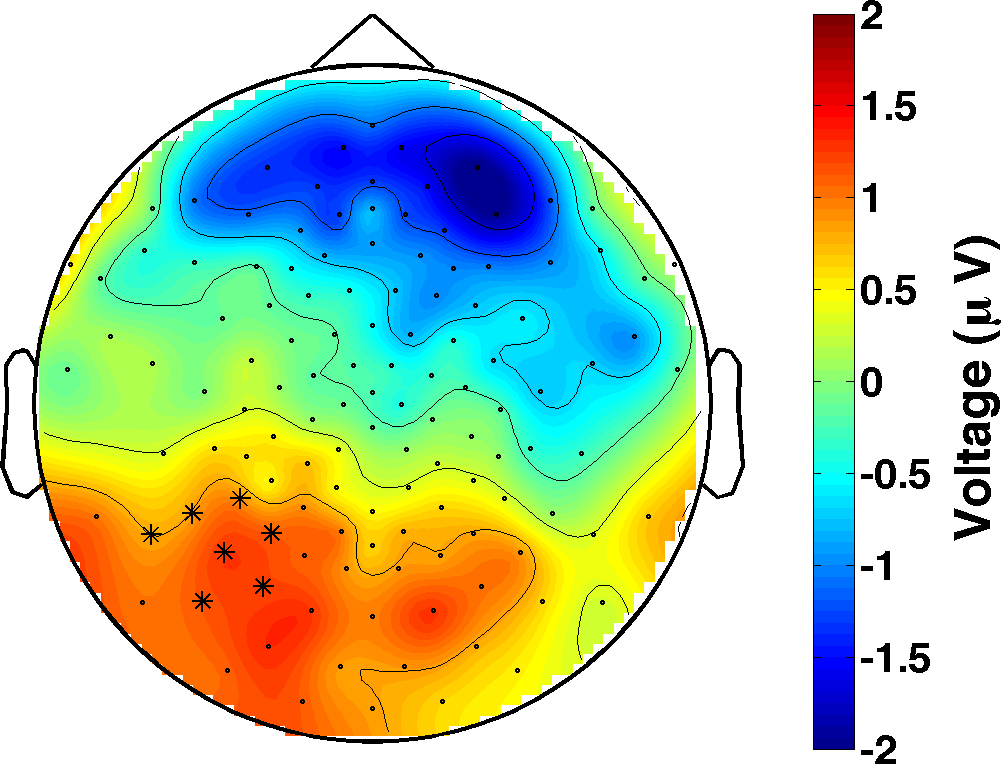
\includegraphics[width=.29\textwidth]{./figs/exp1/tla_topocont_ga_word_RgH_rc_mass_p2vsword_RgH_rc_spac_p2_E50_E51_E57_E58_E59_E64_E65_122_222_-2p0_2p0_cb} &
  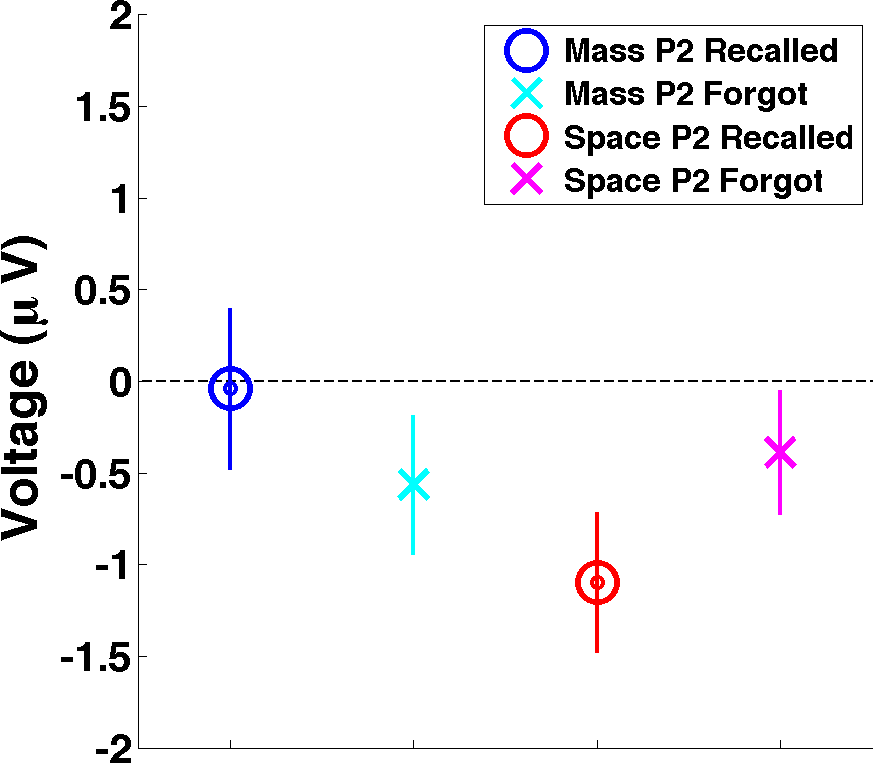
\includegraphics[width=.30\textwidth]{./figs/exp1/tla_line_ga_word_RgH_rc_mass_p2_word_RgH_fo_mass_p2_word_RgH_rc_spac_p2_word_RgH_fo_spac_p2_E50_E51_E57_E58_E59_E64_E65_122_222_ylabel} \\
  \end{tabular}
  \caption{N1 to words at electrode 58 (T5) and neighbors, analyzed window 122--222~ms: (a) Massed ERPs; (b) spaced ERPs; (c) contrast between subsequently recalled massed \textit{vs.} spaced Presentation 2 (P2) across time and electrodes (*); (d) analyzed means (error bars are SEM).  The early negative peak is significantly larger for spaced compared to massed repetitions.}
  \label{fig:N1}
  %Figure~\ref{fig:N1}
\end{figure}

If attention is modulated by spacing, early ERP components may show effects.  The visual N1 typically shows effects of selective attention, making this component particularly relevant to deficient processing.
% particularly during discrimination tasks \cite{VogeLuck2000}.  In the present paradigm participants do not make responses during encoding, but perhaps a difference will exist if deficient processing of massed items occurs.
A three-way ANOVA with factors of spacing, presentation, and subsequent memory was performed.
A crossover pattern was borne out in the significant three-way interaction [$F(1,22)=10.5$, $p<.005$] that showed spacing and subsequent memory only had effects for repetitions, not for initial presentations.  Recalled spaced repetitions ($M=-1.1~\mu$V) were more negative than forgotten spaced repetitions ($M=-0.39~\mu$V) [$t(22)=2.73$, $p<.05$], recalled massed repetitions ($M=-0.04~\mu$V) [$t(22)=4.37$, $p<.0005$], and (marginally) forgotten massed repetitions ($M=-0.56~\mu$V) [$t(22)=2.039$, $p=.053$].
% Additionally, recalled massed repetitions were marginally more positive than forgotten [$t(22)=1.97$, $p=.06$] (in the opposite direction of spaced repetitions).

% plot: N400 at Cz + surround
\begin{figure}[hp]
  \centering
  \begin{tabular}{cc}
  Massed & Spaced \\
  \multicolumn{1}{l}{(a)} & \multicolumn{1}{l}{(b)} \\
  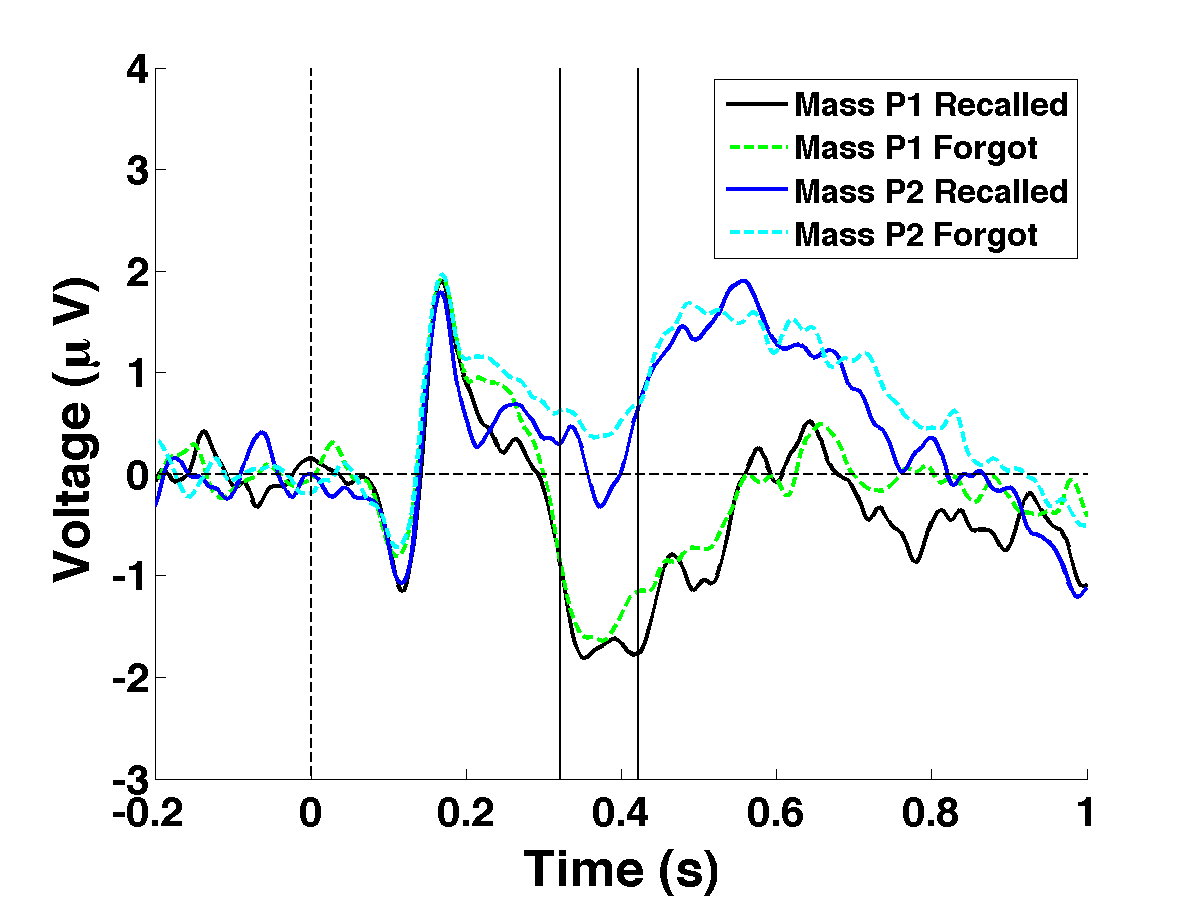
\includegraphics[width=.35\textwidth]{./figs/exp1/tla_single_ga_word_RgH_rc_mass_p1_word_RgH_fo_mass_p1_word_RgH_rc_mass_p2_word_RgH_fo_mass_p2_C_-200_1000_legend_xylabel} &
  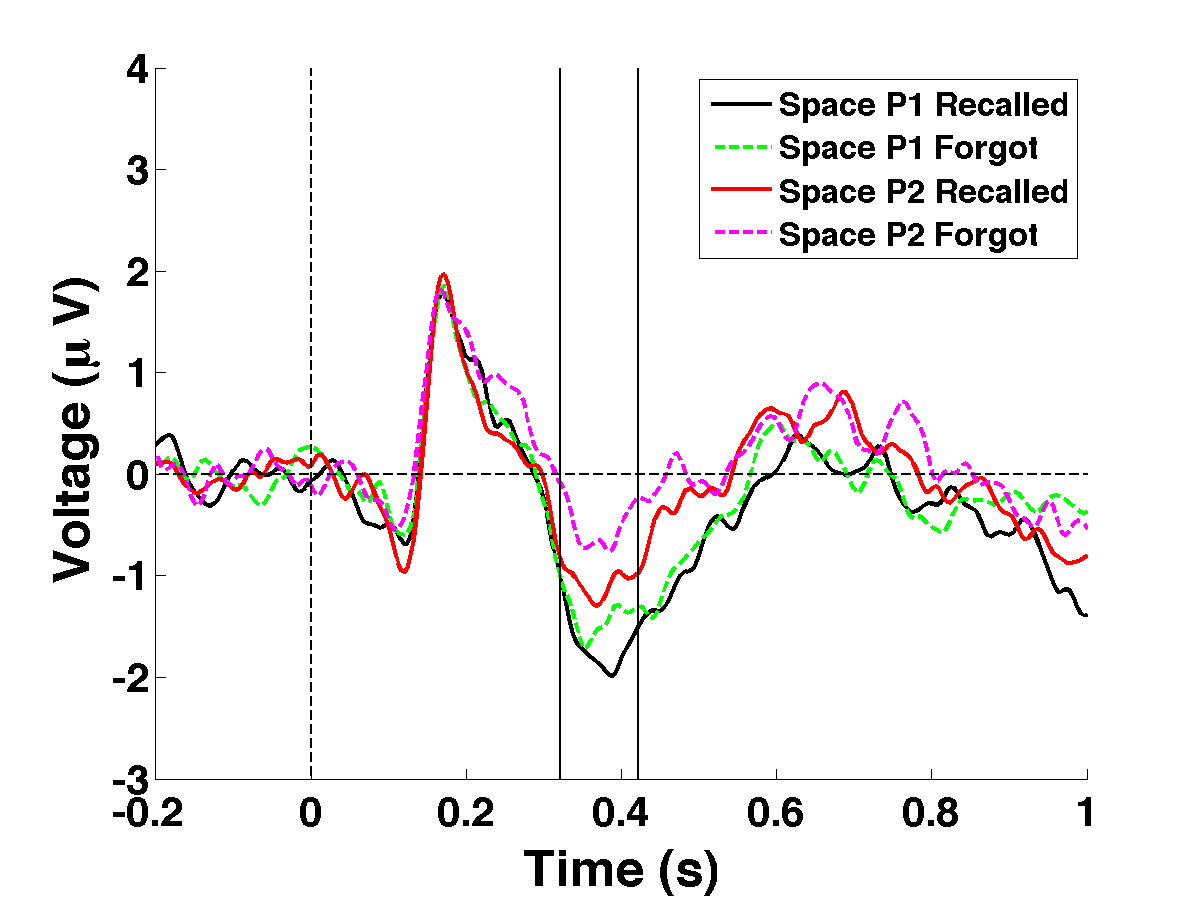
\includegraphics[width=.35\textwidth]{./figs/exp1/tla_single_ga_word_RgH_rc_spac_p1_word_RgH_fo_spac_p1_word_RgH_rc_spac_p2_word_RgH_fo_spac_p2_C_-200_1000_legend_xylabel} \\
  Recalled P2: Massed $-$ Spaced & Means \\
  \multicolumn{1}{l}{(c)} & \multicolumn{1}{l}{(d)} \\
  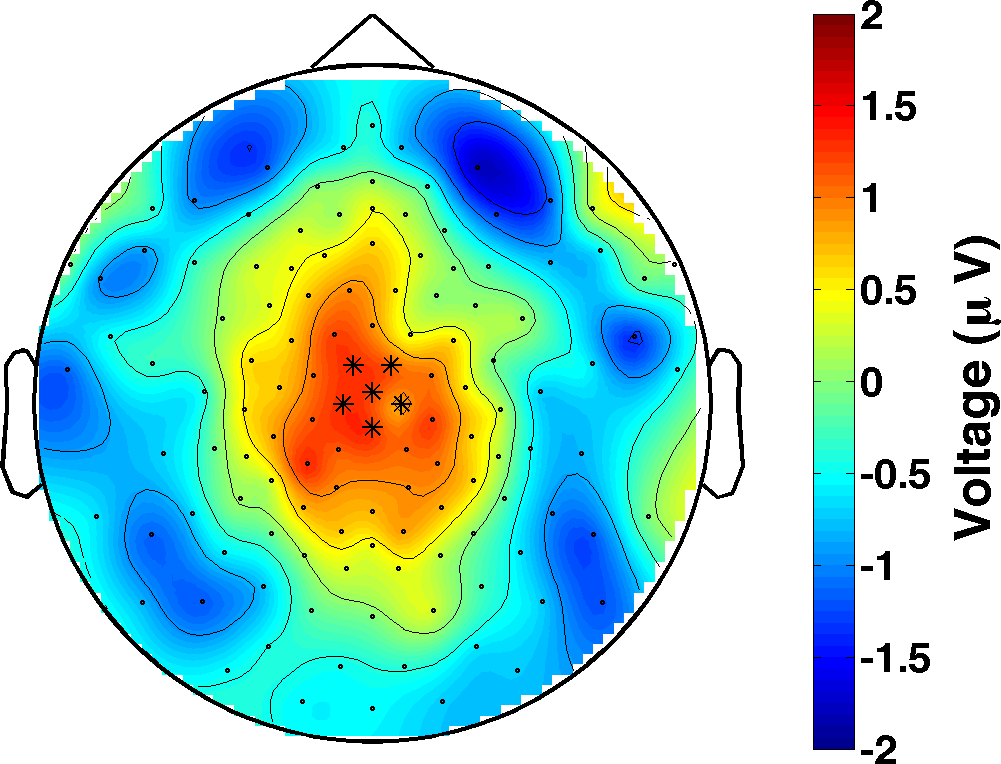
\includegraphics[width=.29\textwidth]{./figs/exp1/tla_topocont_ga_word_RgH_rc_mass_p2vsword_RgH_rc_spac_p2_C_322_422_-2p0_2p0_cb} &
  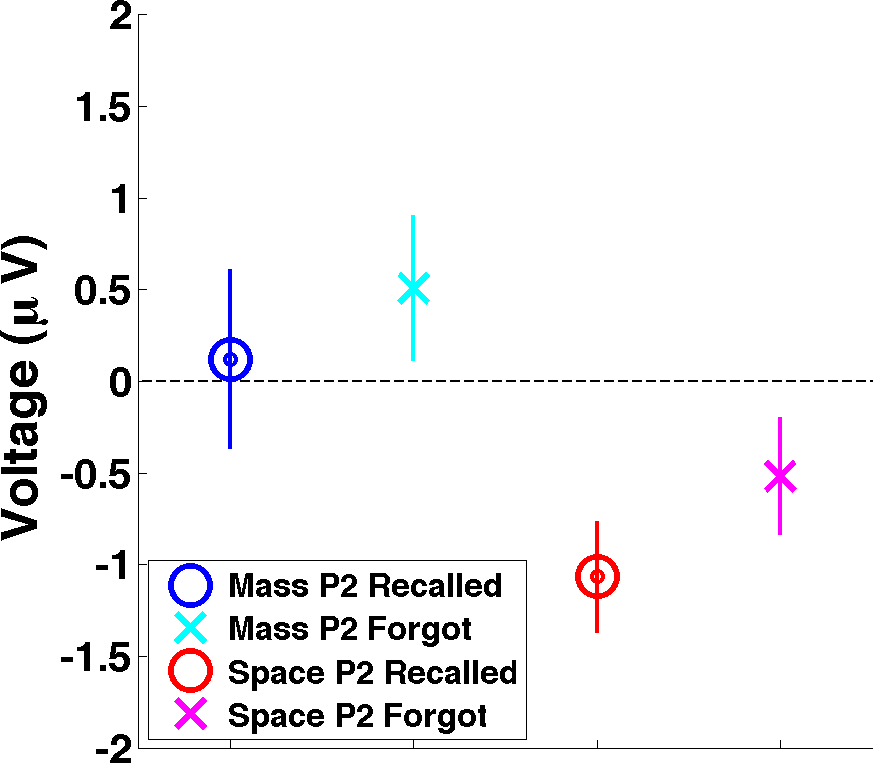
\includegraphics[width=.30\textwidth]{./figs/exp1/tla_line_ga_word_RgH_rc_mass_p2_word_RgH_fo_mass_p2_word_RgH_rc_spac_p2_word_RgH_fo_spac_p2_C_322_422_ylabel} \\
  \end{tabular}
  \caption{N400 to words at electrode Cz and neighbors, analyzed window 322--422~ms: (a) Massed ERPs; (b) spaced ERPs; (c) contrast between subsequently recalled massed \textit{vs.} spaced Presentation 2 (P2) across time and electrodes (*); (d) analyzed means (error bars are SEM).  The negative peak at 400~ms is significantly smaller for massed compared to spaced repetitions.}
  \label{fig:N400}
  %Figure~\ref{fig:N400}
\end{figure}

% % plot: LPC at E60 + surround and E85 + surround

% \begin{figure}
%   \centering
%   \begin{tabular}{ccc}
%   & Left & Right \\
%   \raisebox{2.2cm}{\rotatebox{90}{Massed}} & \includegraphics[width=.45\textwidth]{./figs/exp1/tla_single_ga_word_RgH_rc_mass_p1_word_RgH_fo_mass_p1_word_RgH_rc_mass_p2_word_RgH_fo_mass_p2_LPS2_-200_1000_legend_xylabel} &
%   \includegraphics[width=.45\textwidth]{./figs/exp1/tla_single_ga_word_RgH_rc_mass_p1_word_RgH_fo_mass_p1_word_RgH_rc_mass_p2_word_RgH_fo_mass_p2_RPS2_-200_1000_legend_xylabel} \\
%   \raisebox{2.2cm}{\rotatebox{90}{Spaced}} & \includegraphics[width=.45\textwidth]{./figs/exp1/tla_single_ga_word_RgH_rc_spac_p1_word_RgH_fo_spac_p1_word_RgH_rc_spac_p2_word_RgH_fo_spac_p2_LPS2_-200_1000_legend_xylabel} &
%   \includegraphics[width=.45\textwidth]{./figs/exp1/tla_single_ga_word_RgH_rc_spac_p1_word_RgH_fo_spac_p1_word_RgH_rc_spac_p2_word_RgH_fo_spac_p2_RPS2_-200_1000_legend_xylabel} \\
%   \end{tabular}
%   \caption{LPC to words at electrodes 60 (left) and 85 (right) and neighbors: Massed (top) and spaced (bottom).  The positive peak around 600~ms is significantly larger for massed compared to spaced repetitions.}
%   \label{fig:LPC}
%   %Figure~\ref{fig:LPC}
% \end{figure}

% For the N400 latency ANOVA, there was an interaction between spacing and presentation [$F(1,26)=4.73$, $p<.05$] such that massed repetitions (presentation 2; $M=346$~ms) occurred about 20~ms earlier than all other conditions; this is slightly different from the 1-way ANOVA results where both massed and spaced repetitions peaked earlier than single presentations items.

If the spacing effect results from differences in semantic priming and processing, the N400 should show effects.
For voltage, a significant spacing $\times$ presentation interaction showed a graded pattern [$F(1,22)=12.4$, $p<.01$]: voltage becomes more negative from massed repetition to spaced repetition to first presentation [$p$s~$<.01$].  Contributing to this were main effects of spacing [$F(1,22)=9.65, p=.00514$] and presentation [$F(1,22)=30.8, p=1.42e^{-5}$]; spaced items were more negative, and repetitions were less negative.  There was also a main effect of memory [$F(1,22)=4.47$, $p<.05$]: remembered items ($M=-1.06~\mu$V) were more negative than forgotten ones ($M=-0.71~\mu$V).
\cbstart There were no other interactions, but pairwise comparisons from the three-way interaction showed that, while there were no differences for the initial presentations, remembered spaced repetitions ($M=-1.07~\mu$V) were more negative than forgotten spaced repetitions ($M=-0.52~\mu$V) [$p<.05$] and both remembered ($M=0.12~\mu$V) and forgotten ($M=0.51~\mu$V) massed repetitions [$p$s~$<.01$].\cbend
% Here, the most interesting pairwise comparisons showed that for repetitions, forgotten massed items ($M=1.1~\mu$V) were more positive than remembered ones ($M=0.55~\mu$V), and each was more positive than both spaced forgotten ($M=-0.16~\mu$V) and spaced recalled ($M=-0.34~\mu$V) repetitions [$p$s~$<.05$].
No effects of latency were found.

% plot: LPC at E77 + surround
\begin{figure}[hp]
  \centering
  \begin{tabular}{cc}
  Massed & Spaced \\
  \multicolumn{1}{l}{(a)} & \multicolumn{1}{l}{(b)} \\
  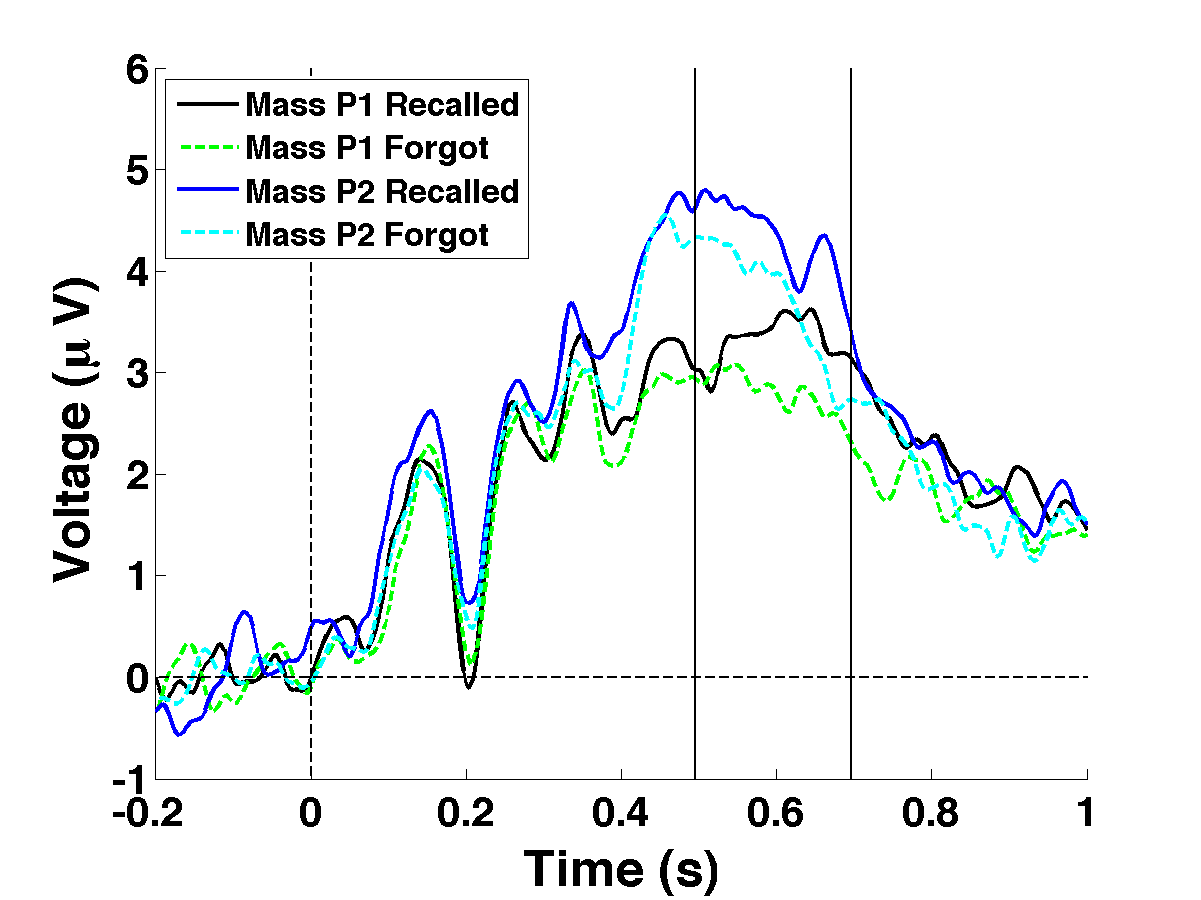
\includegraphics[width=.35\textwidth]{./figs/exp1/tla_single_ga_word_RgH_rc_mass_p1_word_RgH_fo_mass_p1_word_RgH_rc_mass_p2_word_RgH_fo_mass_p2_E62_E72_E76_E77_E78_E84_E85_-200_1000_legend_xylabel} &
  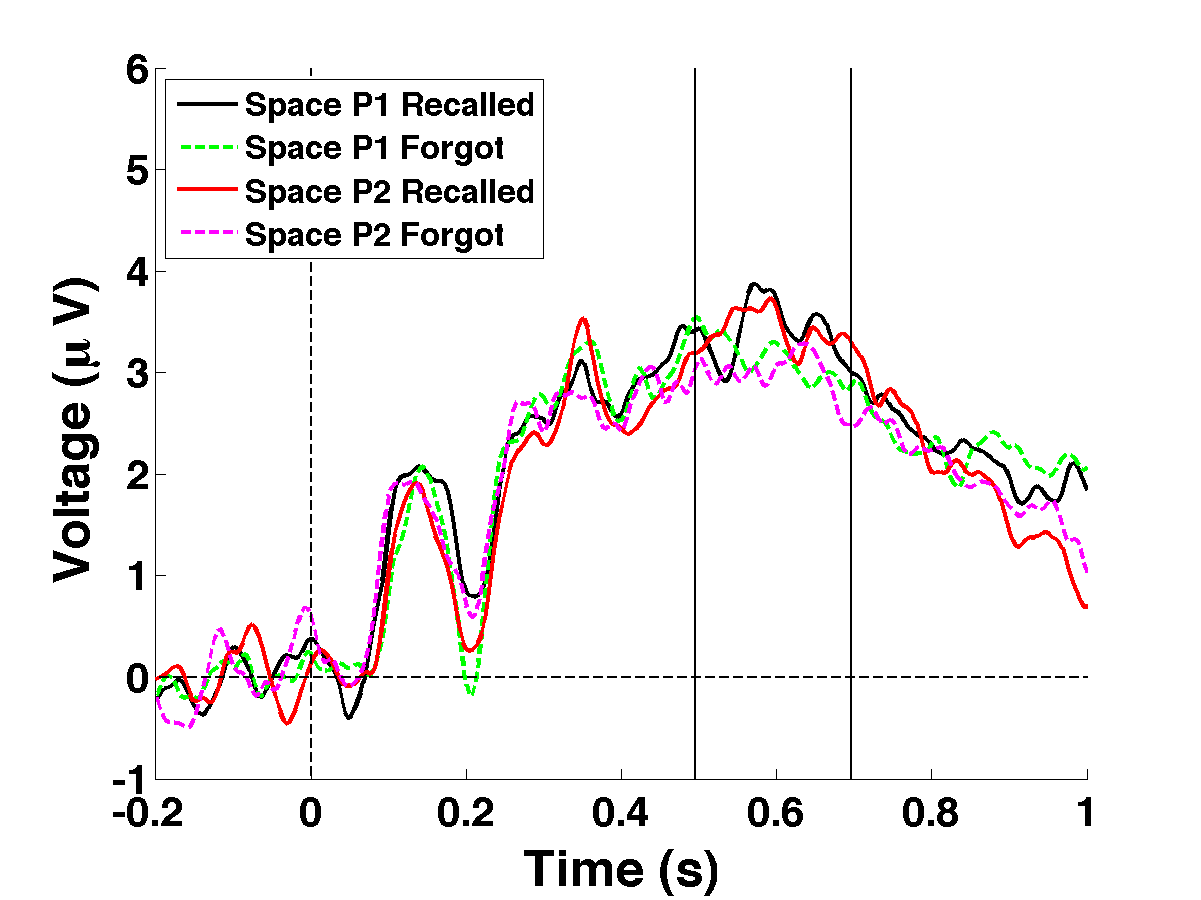
\includegraphics[width=.35\textwidth]{./figs/exp1/tla_single_ga_word_RgH_rc_spac_p1_word_RgH_fo_spac_p1_word_RgH_rc_spac_p2_word_RgH_fo_spac_p2_E62_E72_E76_E77_E78_E84_E85_-200_1000_legend_xylabel} \\
  Recalled P2: Massed $-$ Spaced & Means \\
  \multicolumn{1}{l}{(c)} & \multicolumn{1}{l}{(d)} \\
  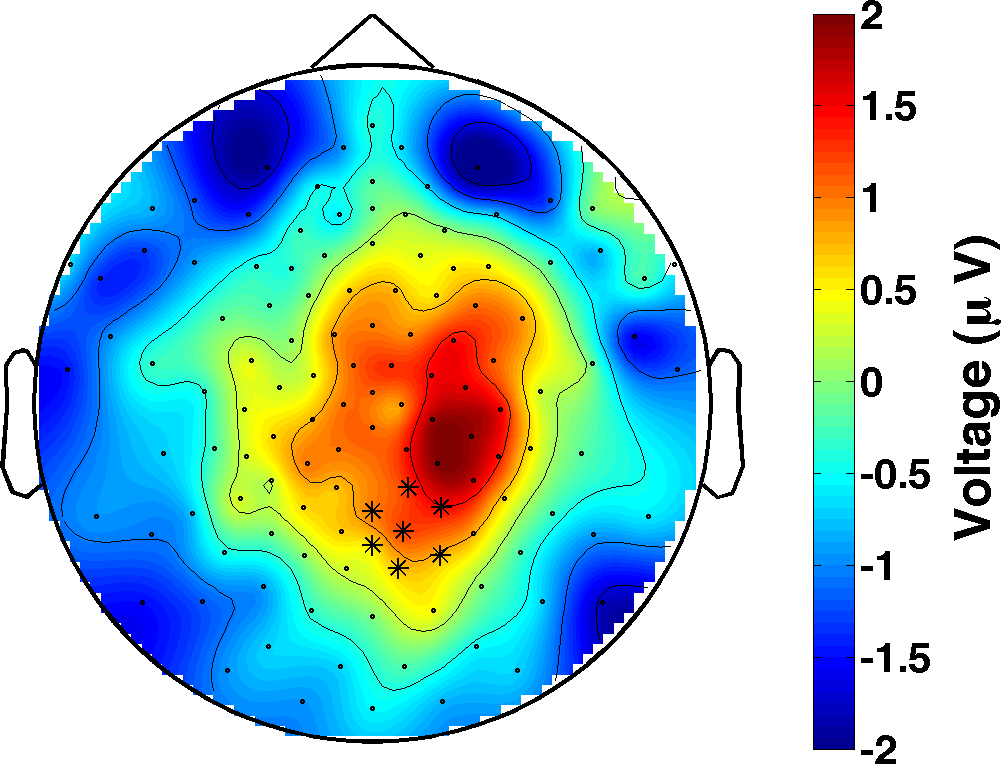
\includegraphics[width=.29\textwidth]{./figs/exp1/tla_topocont_ga_word_RgH_rc_mass_p2vsword_RgH_rc_spac_p2_E62_E72_E76_E77_E78_E84_E85_496_696_-2p0_2p0_cb} &
  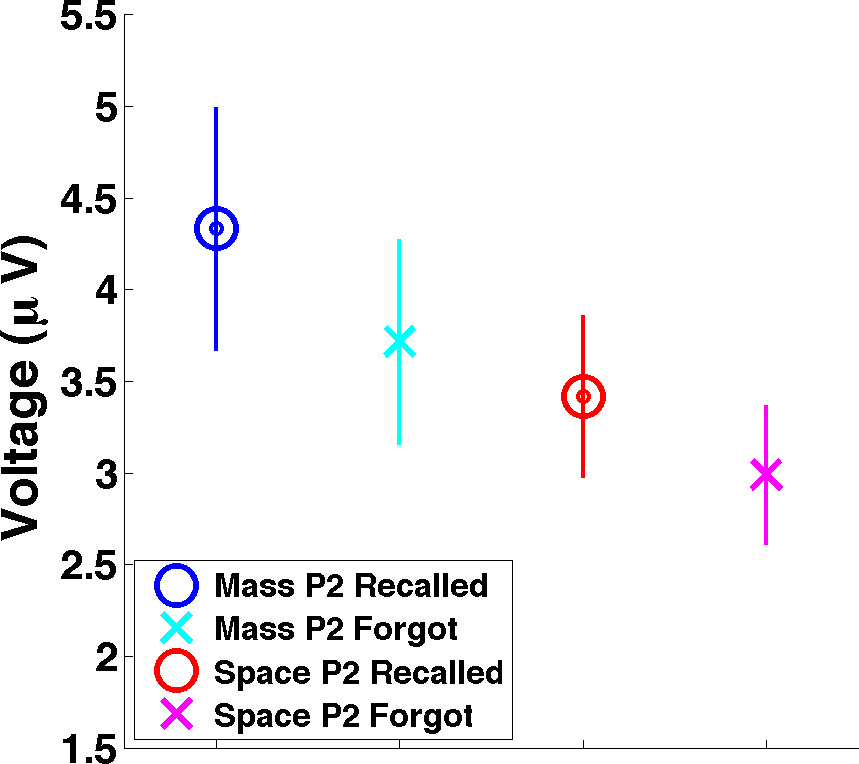
\includegraphics[width=.30\textwidth]{./figs/exp1/tla_line_ga_word_RgH_rc_mass_p2_word_RgH_fo_mass_p2_word_RgH_rc_spac_p2_word_RgH_fo_spac_p2_E62_E72_E76_E77_E78_E84_E85_496_696_ylabel} \\
  \end{tabular}
  \caption{LPC to words at electrode 77 and neighbors, analyzed window 496--696~ms: (a) Massed ERPs; (b) spaced ERPs; (c) contrast between subsequently recalled massed \textit{vs.} spaced Presentation 2 (P2) across time and electrodes (*); (d) analyzed means (error bars are SEM).  The positive peak around 600~ms is significantly larger for massed compared to spaced repetitions.}
  \label{fig:LPC}
  %Figure~\ref{fig:LPC}
\end{figure}

% Since our experimental design was different from that of \citeA{VanSEtal2007}, we performed two tests.
% A 1-way ANOVA for spacing (spaced and massed repetitions and single/first presentation) was performed with the dependent variable of peak latency.  So as not to ignore single presentation trials (which were not tested), we combined the first presentation of spaced and massed items with the single presentation items.  There were no N400 differences.  The LPC showed a marginal interaction [$F(2,44)=3.02, p=.059$] with significant pairwise comparisons.  The peak for massed repetitions ($M=562$~ms) occurred about 30~ms earlier than both single presentations ($M=588$~ms) [$t(22)=2.19$, $p<.05$] and spaced ($M=589$~ms) repetitions [$t(22)=2.13$, $p<.05$].
% This replicated previous results, though with smaller peak differences between all conditions.

% A similar ANOVA was performed for voltage averaged across the analysis window surrounding the average peak.  The N400 showed a graded pattern in which single presentations ($M=-1.47~\mu$V) were more negative than both spaced ($M=-0.79~\mu$V) [$t(22)=3.9$, $p<.001$] and massed ($M=0.32~\mu$V) [$t(22)=5.19$, $p<.00005$] repetitions, and spaced were more negative than massed [$t(22)=4.42$, $p<.001$].
% % This replicates their pattern, though they do not report pairwise statistics.
% For the LPC effect, massed repetitions ($M=4.02~\mu$V) were more positive than both spaced ($M=3.2\mu$V) [$t(22)=2.26$, $p<.05$] and single presentations ($M=3.21~\mu$V) [$t(22)=2.24, p<.05$].
% % Here, we do not replicate an effect for spaced compared to single/first presentations.

The LPC has been linked to conscious stimulus recognition in repetition paradigms, and may also show subsequent memory effects if the retrieval of information helps long-term memory performance.
For voltage, there was a significant interaction of spacing $\times$ presentation [$F(1,22)=5.38$, $p<.05$].  Massed repetitions ($M=4.02~\mu$V) were more positive than all other conditions (spaced repetition: $M=3.2~\mu$V; massed initial: $M=3.06~\mu$V [$p$s~$<.05$]; marginal for spaced initial: $M=3.27~\mu$V [$p=.055$]).  Additionally, there was a main effect of memory for voltage, showing a typical subsequent memory effect: recalled ($M=3.62~\mu$V) were more positive than forgotten ($M=3.16~\mu$V).

\hl{(TODO: examine where the main effect of memory comes from)}

Examining the latency of the LPC peak, there was a significant interaction of spacing $\times$ presentation [$F(1,22)=5.83$, $p<.05$].  Massed repetitions ($M=564$~ms) peaked earlier than all other conditions (spaced repetition: $M=597$~ms; massed initial: $M=597$~ms; spaced initial: $M=587$~ms [$p$s~$<.05$]).    

% There was also a marginal main effect of memory for latency [$F(1,26)=2.96$, $p=.097$].  Subsequently recalled items ($M=602$~ms) tended to peak later than those that were forgotten ($M=589$~ms).  This is probably influenced by spaced repetitions peaking later and memory being better for spaced items on average.

\subsection{ERP discussion}

The N1 showed that recalled spaced word repetitions were more negative compared to the other conditions (repetitions of recalled massed words and forgotten spaced and massed words), which can be interpreted to mean that they received the most attention.
% The pattern for subsequently recalled \textit{vs.} forgotten spaced repetitions indicates that a larger N1 means more attention was paid to that item.
Massed items are at a disadvantage compared to remembered spaced items, supporting the deficient processing hypothesis.  Because remembered massed items are the least negative but are still remembered later, there are likely other mechanisms that influence memory encoding in addition to attention.  This implies that attentional processing affects subsequent memory differently for massed and spaced items.
% Regardless, this is an interesting effect because the visual N1 does not typically show subsequent memory effects \cite<e.g.,>{CurrEtal2002,DuarEtal2004,DuarEtal2006}.
% Even if these attention effects are key, this cannot be the whole story behind the spacing effect; otherwise there would have been a main effect of spacing [$F(1,22)=3.05$, $p=.095$].

% \hl{Actually, there should be a spacing x memory interaction, which we do see interact with presentation... reinterpret.}

The N400 is more negative when semantic processes are engaged to a greater extent.  There was a typical repetition effect showing that voltage decreased with repetition lag, and this interacted with presentation (repetitions attenuate but more so for massed).  This implies that semantic processing engages more for spaced than massed repetitions, but not as much as initial presentations.
Because the significant effect of subsequent memory showed that remembered items have greater negative amplitudes, this indicates that more semantic processing occurs for remembered items.  Spaced items seem to have an overall processing advantage, or perhaps massed items have an overall disadvantage due their attenuated N400.  This is all in line with the semantic activation hypothesis of \citeA{Chal1993} and the position taken by \citeA{VanSEtal2007}, and therefore supports the deficient processing theory.

The typical interpretation of the LPC effect is that it is more positive during the retrieval of an item's prior presentation \cite{OlicEtal2000,VanSEtal2007}.  The present results show this positivity for massed repetitions as well as an earlier peak, implying faster retrieval of the initial stimulus presentation compared to spaced repetitions.
% Though spaced repetitions do not show an effect, an (unreported) analysis over left parietal (more typical for the parietal old/new effect) showed that spaced peaked later
% Surely spaced items were not forgotten even though they did not show an LPC effect, so this effect must not be indexing recollection (which makes sense when comparing its topography to that of the parietal old/new effect, which is typically more left parietal).
In relation to the N400 results (showing that semantic processing does not need to engage for primed representations), it seems possible that the LPC indexes the information that is in working memory.  This result does not seem to directly support any of the theories, unless the match to working memory is an indicator for processing to disengage (deficient processing).

% Raai2003 p. 442: a short spacing interval keeps the item in STS and hence prevents the strengthening of the LTS trace.

\subsection{Time--frequency results}

Spectral decomposition for time--frequency analyses (no low-pass filter) used a set of $38$ Morlet wavelets that were logarithmically spaced from $3$ to $80$~Hz; each wavelet had a width of $6$ cycles.  Trials were down-sampled to $50$~Hz after calculating power and were z-transformed relative to the distribution of all word stimuli with a reference time of $-300$ to $-100$~ms relative to stimulus onset.
Only the pre-stimulus periods for words were used because the analogous reference time for images would be while words were on the screen.
The following frequency bands were analyzed: theta ($4.1$ to $7.7$~Hz); lower alpha ($8.4$ to $10.1$~Hz); upper alpha ($11$ to $12$~Hz); lower beta ($13.1$ to $20.5$~Hz); upper beta ($22.4$ to $29.2$~Hz); lower gamma ($31.9$ to $45.5$~Hz); upper gamma ($49.7$ to $77.4$~Hz).

Time--frequency differences were assessed using repeated measures ANOVAs due to the large number of factors, but because the effect topographies are not as well defined as in ERP analyses a cluster-based permutation test \cite{MariOost2007} was used as the basis for electrode choice.  Clustering was done by performing a $t$-test for conditions of interest within each time/electrode bin across subjects, followed by grouping together the adjacent bins which yielded a $p$-value of less than $.05$.  Significant differences between pairwise conditions (spaced/massed repetitions, subsequently recalled/forgotten; run separately for words and images) were calculated using a Monte Carlo-style permutation test of the summed $t$-values within a given cluster.  Each observed cluster was subject to 500 random permutations of condition labels where its significance was estimated by the proportion of random permutations which yielded clusters that had a summed $t$-value as large or larger than the observed cluster.  A given electrode for a given frequency band was included in the analysis if it showed a significant difference in at least two of the six pairwise contrasts.  The resulting topographies largely agree with those reported in the memory and attention literature cited in the present paper.
% should I do half of the pairwise comparisons instead? maybe later.


% alpha ($8.4$ to $12$~Hz)
% beta ($13.1$ to $29.2$~Hz)
% gamma ($31.9$ to $77.4$~Hz)


Since oscillatory effects can spread out over time (especially at low frequencies), we analyzed images in addition to words.
% because there are no time-locked oscillatory ``components'' \textit{per se} like with ERPs that would be perturbed by image stimuli immediately following words.
Because word and image stimuli are presented successively, we need to consider that different patterns may be expected during these to-be-associated stimuli for spaced and massed repetitions.  During a repetition trial, there is the potential for both episodic memory, attentional processes, and semantic processes to occur, perhaps at the same time.  Using reverse inference, these can be examined by frequency band (theta, lower alpha, and upper alpha and lower beta, respectively).

Three-way ANOVAs with factors of spacing (spaced and massed), subsequent memory (recalled and forgotten), and time (0--500~ms and 500--1000~ms) were performed for word and image repetitions on power in the theta, lower alpha, upper alpha, and lower beta bands (eight ANOVAs).  The two types of stimuli were analyzed separately because their time courses are not necessarily comparable.  Only repetition events were analyzed.

% \hl{(Why only analyze repetition events? Because including P1 would require slogging through so many stats that aren't that interesting. But I should look at them again.  Or write, it was clear from ERP analyses that P2 is where the action is.)}

% We would not expect differences between the initial presentations of spaced and massed items as the locus of the spacing effect occurs after this point.
% % No differences were found [$F$s~$<1.0$].
% There may exist subsequent memory effects here, though it would be difficult to know whether neural activity during the first presentation is the reason for this effect (e.g., perhaps a subsequently remembered item was encoded poorly on the first presentation and very well on the second presentation).  Thus, analyses will focus on the second presentation (the repetition).


% plot: word and image theta
\begin{figure}[H]
  \centering
  \begin{tabular}{ccccc}
  & Theta power & \multicolumn{2}{c}{Recalled P2: Spaced $-$ Massed} & Means \\
  &  & 0--500~ms & 500--1000~ms \\
  & \multicolumn{1}{l}{(a)} & \multicolumn{1}{l}{(b)} & & \multicolumn{1}{l}{(c)} \\
  \raisebox{1.8cm}{\rotatebox{90}{Word}} & 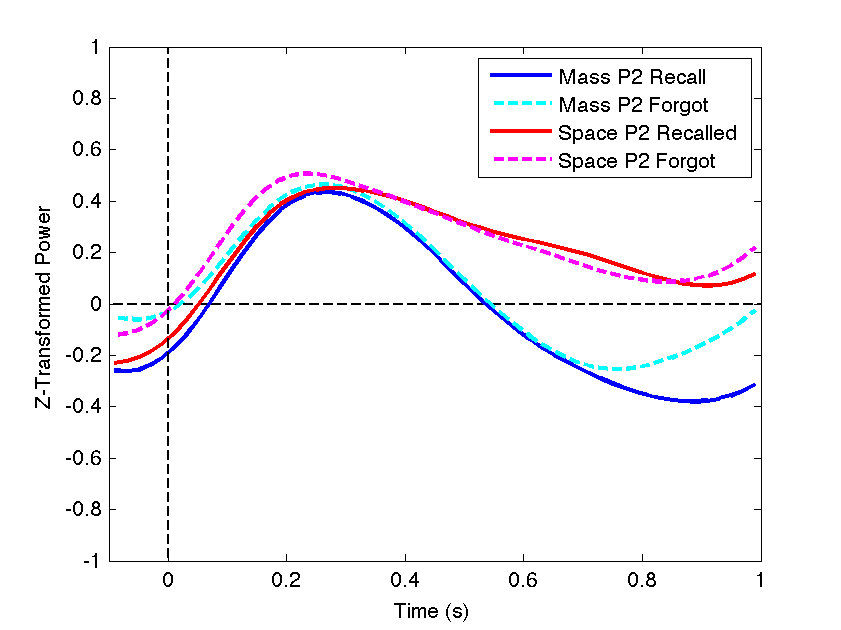
\includegraphics[width=.30\textwidth]{./figs/exp1/tfr_line_ga_word_RgH_rc_mass_p2_word_RgH_fo_mass_p2_word_RgH_rc_spac_p2_word_RgH_fo_spac_p2_89ROIs_-100_1000_4_8_legend} &
  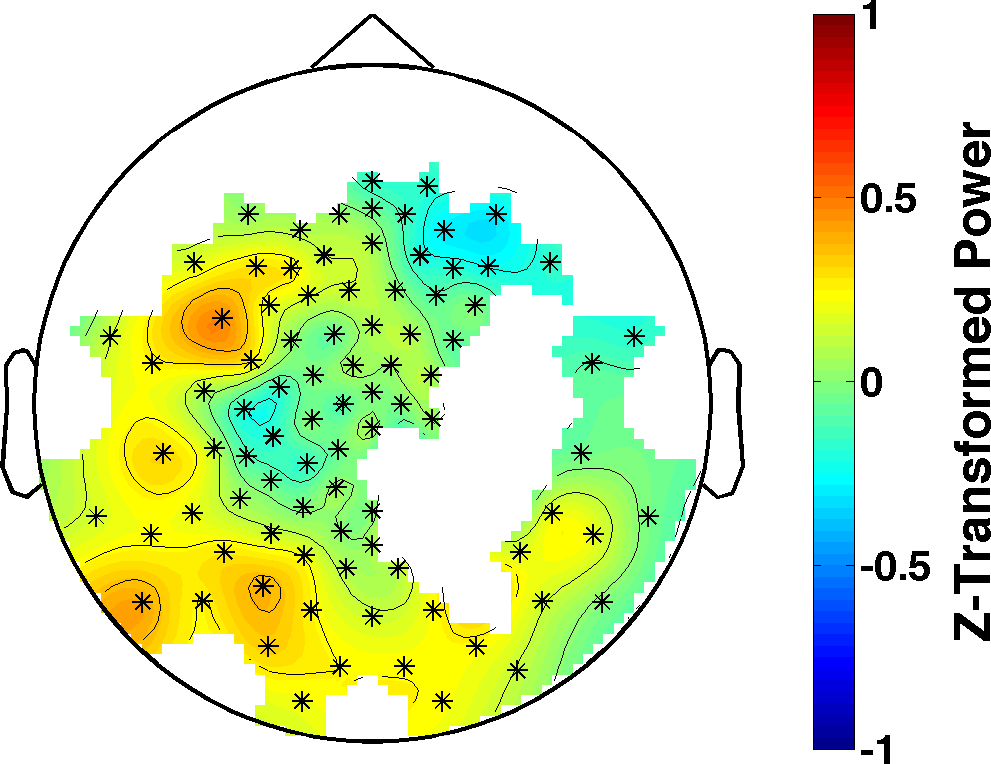
\includegraphics[width=.19\textwidth]{./figs/exp1/tfr_topocont_ga_word_RgH_rc_spac_p2vsword_RgH_rc_mass_p2_89ROIs_4_8_0_500_-1p0_1p0_cb} &
  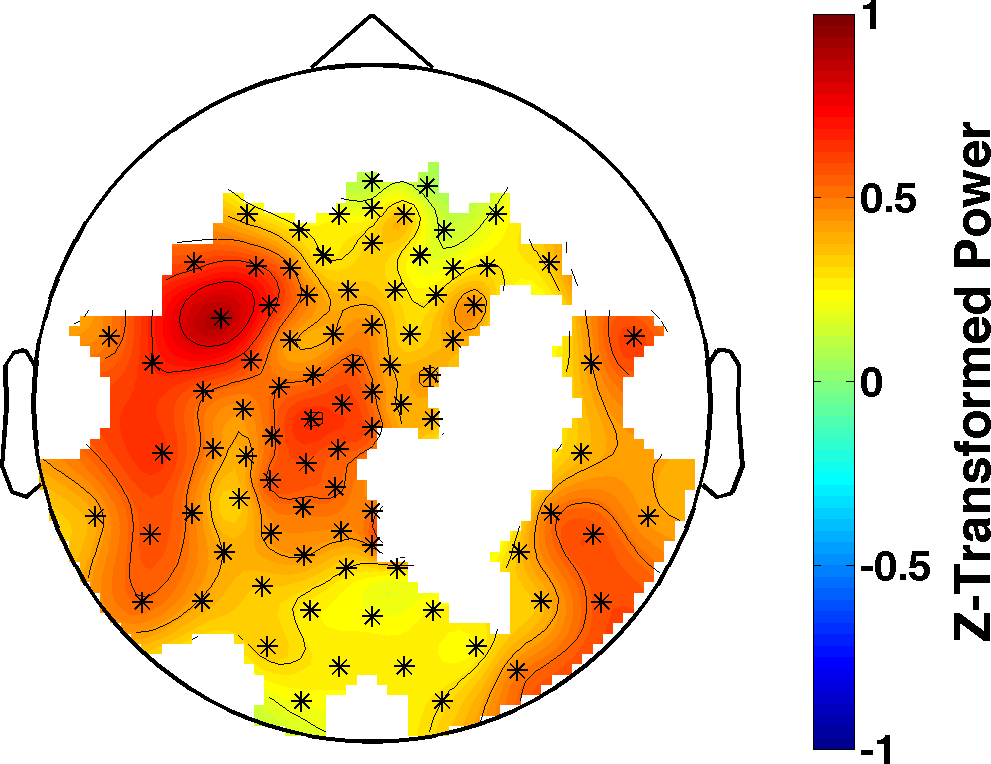
\includegraphics[width=.19\textwidth]{./figs/exp1/tfr_topocont_ga_word_RgH_rc_spac_p2vsword_RgH_rc_mass_p2_89ROIs_4_8_520_1000_-1p0_1p0_cb} &
  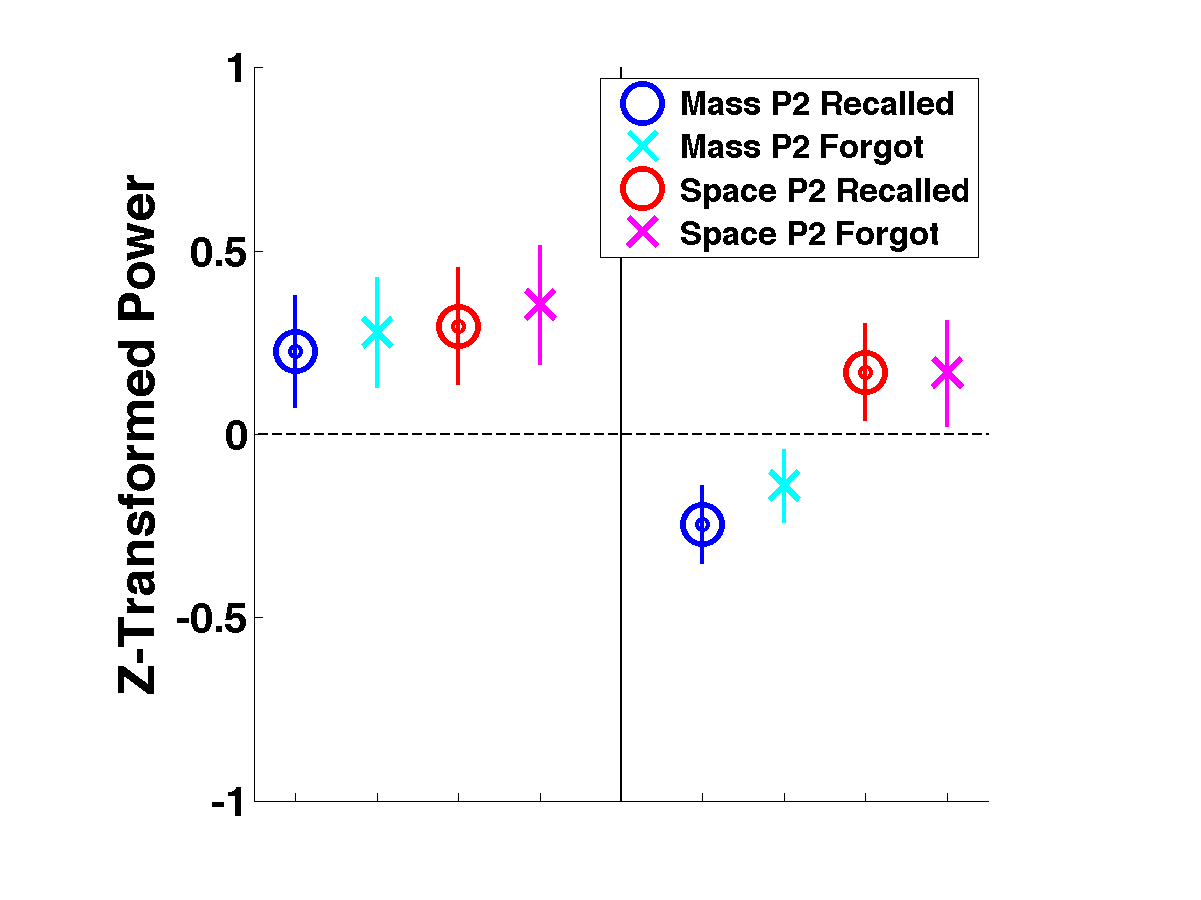
\includegraphics[width=.30\textwidth]{./figs/exp1/tfr_avg_ga_word_RgH_rc_mass_p2_word_RgH_fo_mass_p2_word_RgH_rc_spac_p2_word_RgH_fo_spac_p2_89ROI_0_500_500_1000_4_8_ylabel} \\
  & \multicolumn{1}{l}{(d)} & \multicolumn{1}{l}{(e)} & & \multicolumn{1}{l}{(f)} \\
  \raisebox{1.8cm}{\rotatebox{90}{Image}} & 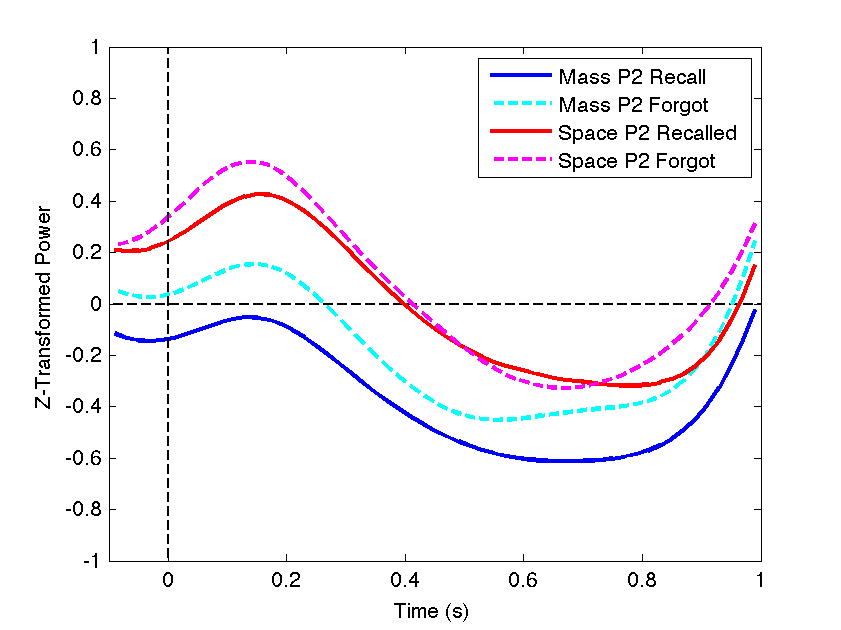
\includegraphics[width=.30\textwidth]{./figs/exp1/tfr_line_ga_img_RgH_rc_mass_p2_img_RgH_fo_mass_p2_img_RgH_rc_spac_p2_img_RgH_fo_spac_p2_99ROIs_-100_1000_4_8_legend} &
  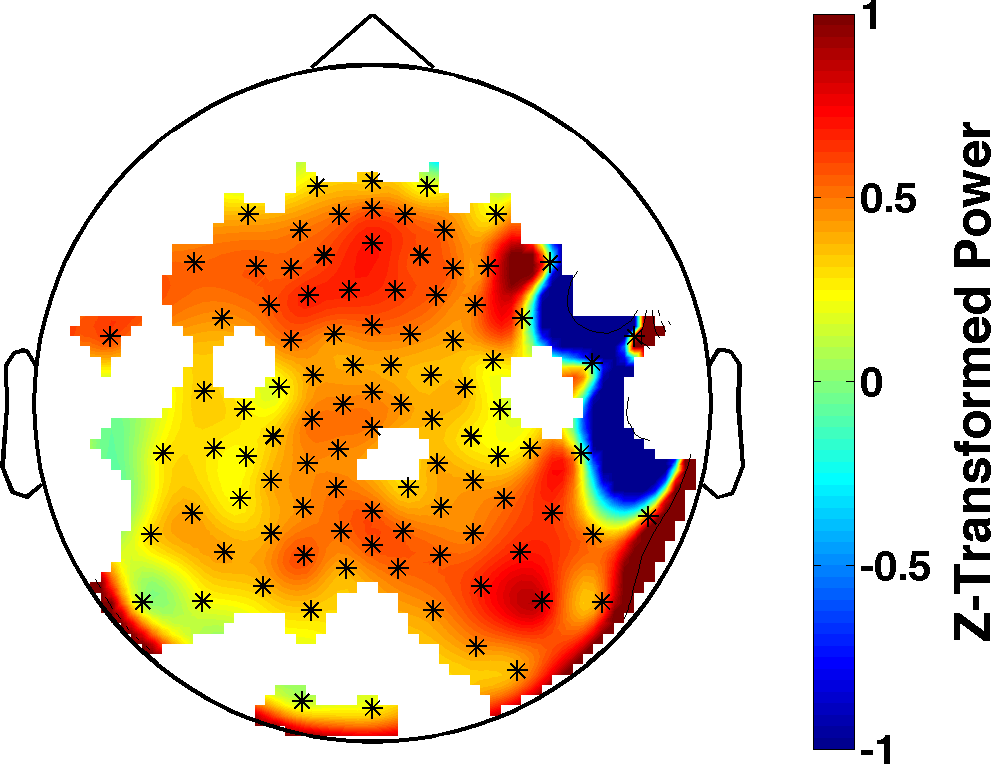
\includegraphics[width=.19\textwidth]{./figs/exp1/tfr_topocont_ga_img_RgH_rc_spac_p2vsimg_RgH_rc_mass_p2_99ROIs_4_8_0_500_-1p0_1p0_cb} &
  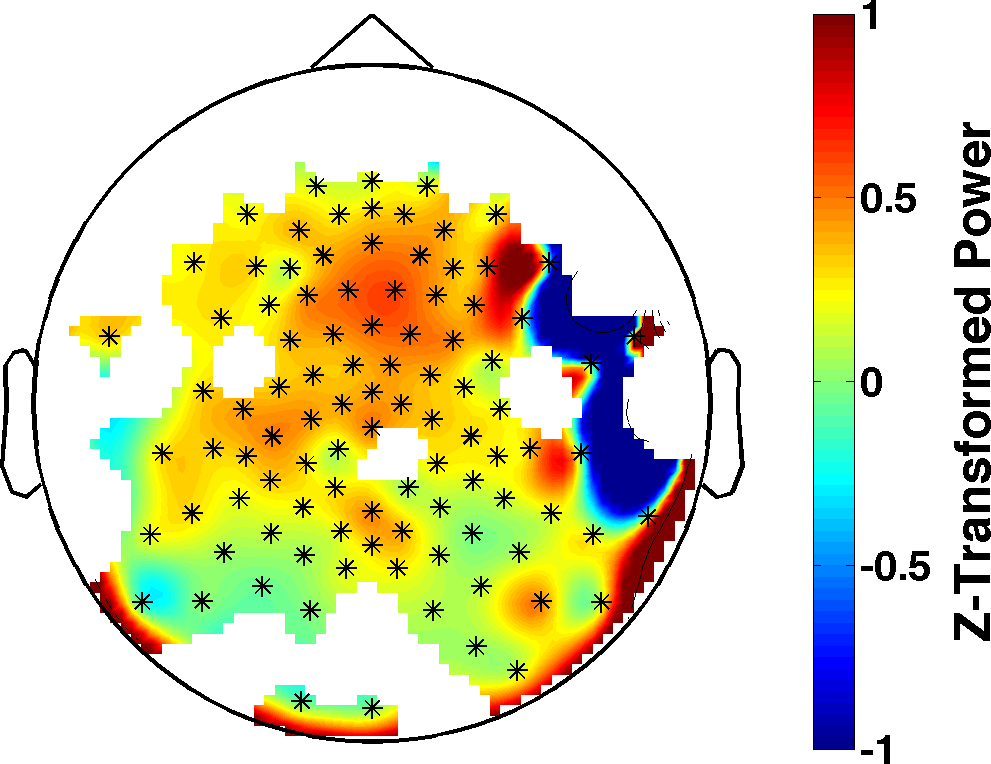
\includegraphics[width=.19\textwidth]{./figs/exp1/tfr_topocont_ga_img_RgH_rc_spac_p2vsimg_RgH_rc_mass_p2_99ROIs_4_8_520_1000_-1p0_1p0_cb} &
  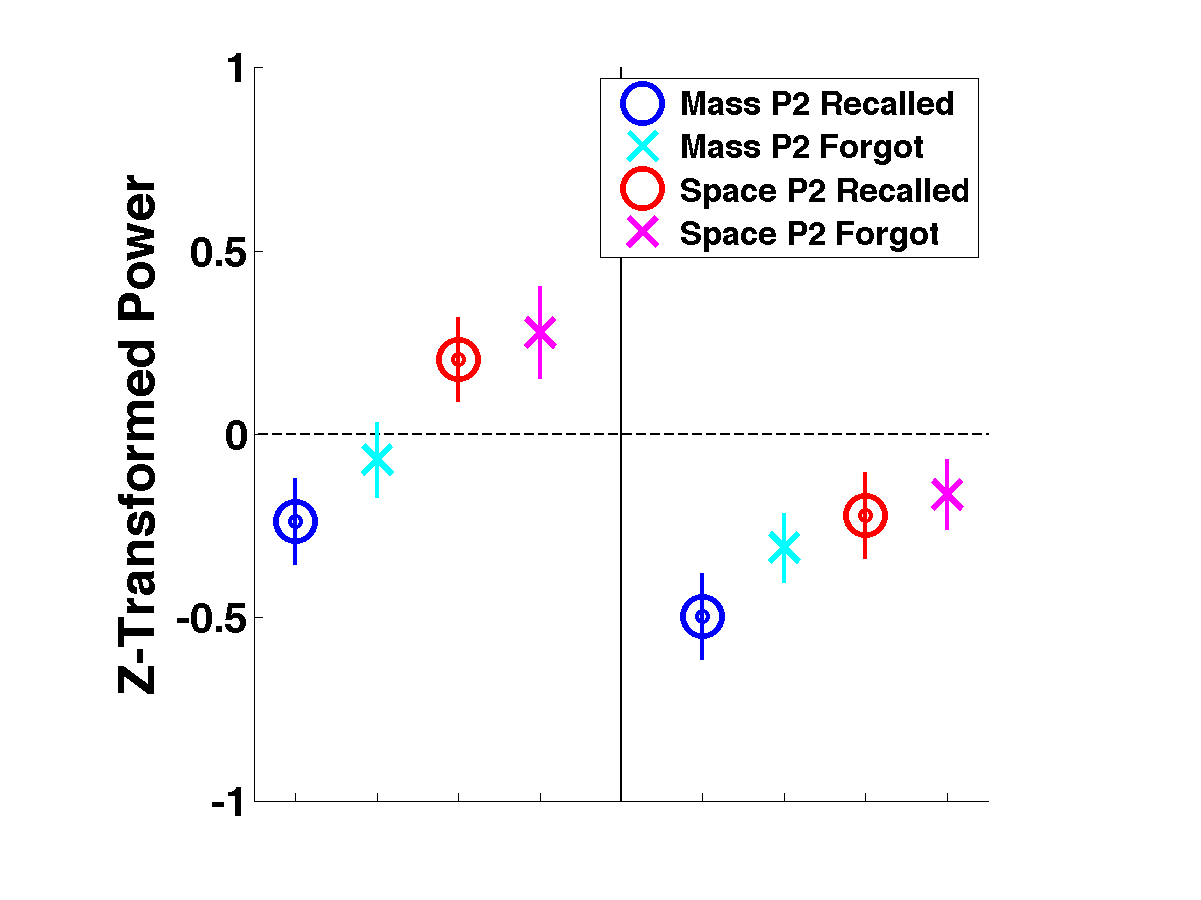
\includegraphics[width=.30\textwidth]{./figs/exp1/tfr_avg_ga_img_RgH_rc_mass_p2_img_RgH_fo_mass_p2_img_RgH_rc_spac_p2_img_RgH_fo_spac_p2_99ROI_0_500_500_1000_4_8_ylabel} \\
  \end{tabular}
  \caption{Theta power to words and images.  (a) and (d) Grand averages; (b) and (e) contrast topographic plot between spaced and massed subsequently recalled trials displaying only the analyzed electrodes (*); (c) and (f) mean values for the two time windows (error bars are SEM).}
  \label{fig:word_img_theta}
  %Figure~\ref{fig:word_img_theta}
\end{figure}

\textit{Word, theta}: Across 89 electrodes (Figure~\ref{fig:word_img_theta}, top), theta showed a spacing $\times$ time interaction [$F(1,22)=26.8, p=3.43e^{-5}$] such that spaced words maintained synchrony across the time windows ($M=0.341$ to $M=0.163$) while massed repetitions showed a power decrease ($M=0.267$ to $M=-0.204$); spaced had greater power than massed in the second time window.
There were main effects of spacing [$F(1,22)=10.3, p=.00399$] and time [$F(1,22)=23.6, p=7.4e^{-5}$] following the same patterns.

\textit{Image, theta}: Across 99 electrodes (Figure~\ref{fig:word_img_theta}, bottom), theta continued to show a spacing $\times$ time interaction [$F(1,22)=6.76, p=.0163$] such that spaced images showed greater power than massed in the first time window ($M=0.239$ \textit{vs.} $M=-0.158$).  Power dropped more for spaced than massed across the time windows: spaced (second window: $M=-0.193$) showed a difference of 0.432 while massed (second window: $M=-0.399$) showed a difference of 0.241.
There were also main effects of spacing [$F(1,22)=31.2, p=1.28e^{-5}$] and time [$F(1,22)=30.6, p=1.46e^{-5}$] following the same patterns, as well as a main effect of memory [$F(1,22)=6.1, p=.0217$] showing that less power is associated with subsequent recall ($M=-0.189$ \textit{vs.} $M=-0.067$; a negative SME).
% (This memory effect is in line with theta indexing memory strength in the short-term store.)

% plot: word and image lower alpha
\begin{figure}[H]
  \centering
  \begin{tabular}{ccccc}
  & Lower alpha power & \multicolumn{2}{c}{Recalled P2: Spaced $-$ Massed} & Means \\
  &  & 0--500~ms & 500--1000~ms \\
  & \multicolumn{1}{l}{(a)} & \multicolumn{1}{l}{(b)} & & \multicolumn{1}{l}{(c)} \\
  \raisebox{1.8cm}{\rotatebox{90}{Word}} & 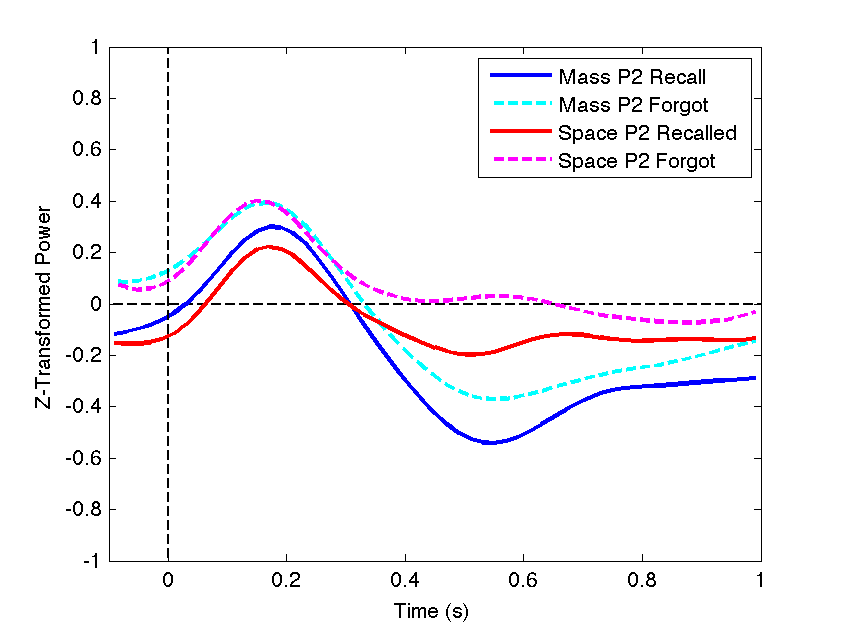
\includegraphics[width=.30\textwidth]{./figs/exp1/tfr_line_ga_word_RgH_rc_mass_p2_word_RgH_fo_mass_p2_word_RgH_rc_spac_p2_word_RgH_fo_spac_p2_101ROIs_-100_1000_8_10_legend} &
  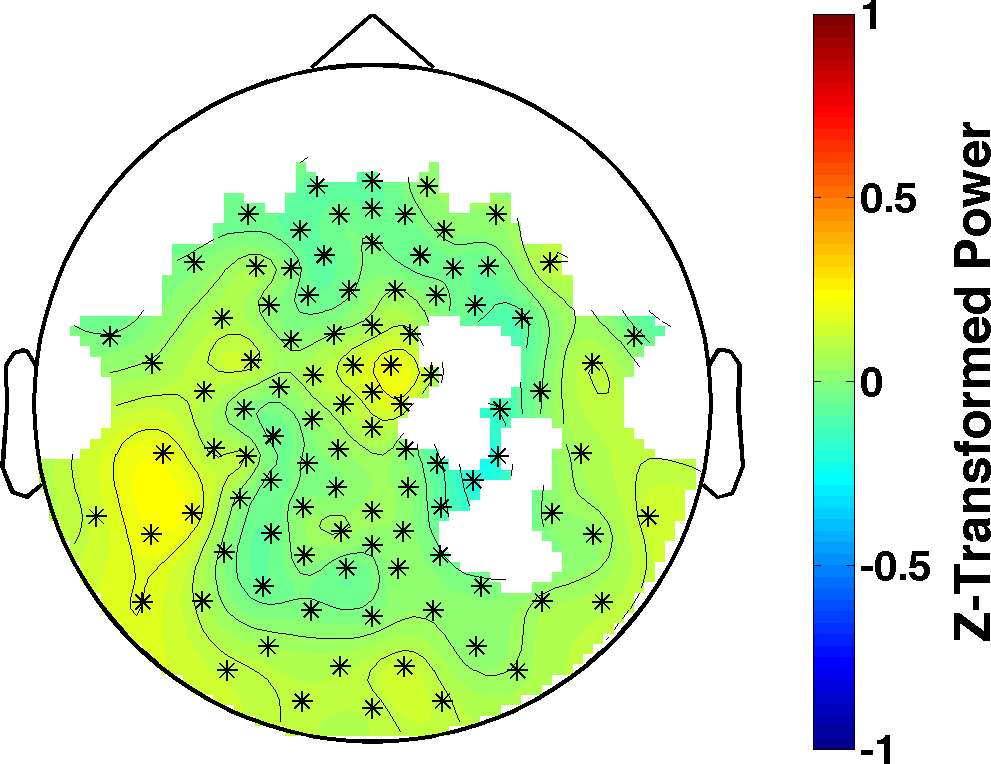
\includegraphics[width=.19\textwidth]{./figs/exp1/tfr_topocont_ga_word_RgH_rc_spac_p2vsword_RgH_rc_mass_p2_101ROIs_8_10_0_500_-1p0_1p0_cb} &
  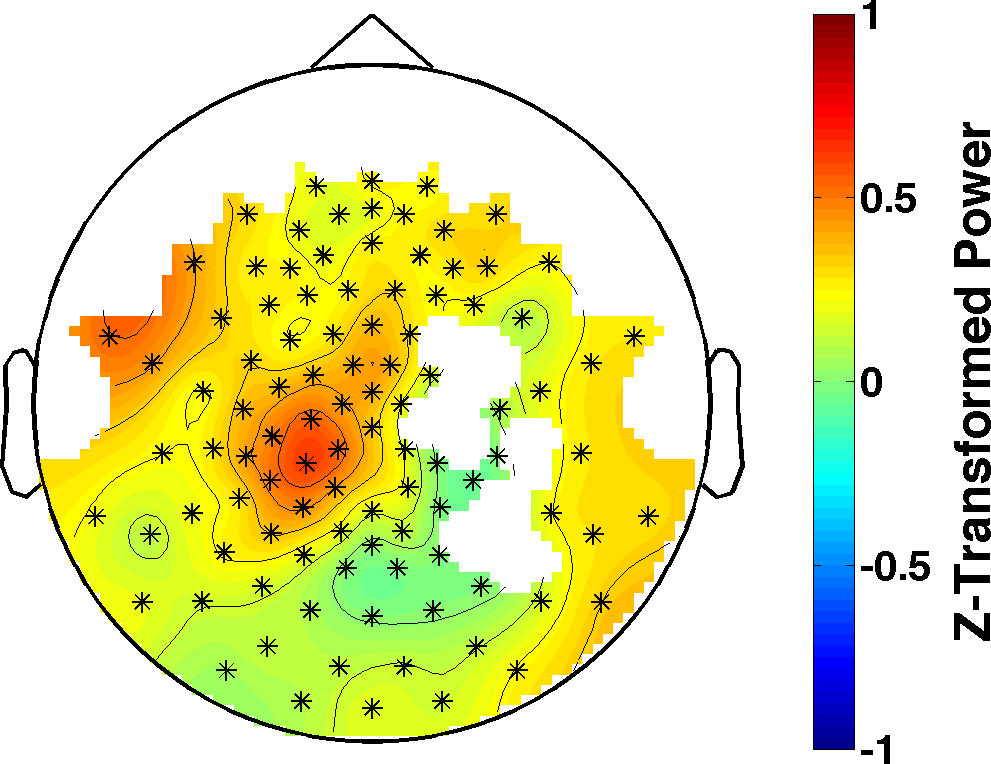
\includegraphics[width=.19\textwidth]{./figs/exp1/tfr_topocont_ga_word_RgH_rc_spac_p2vsword_RgH_rc_mass_p2_101ROIs_8_10_520_1000_-1p0_1p0_cb} &
  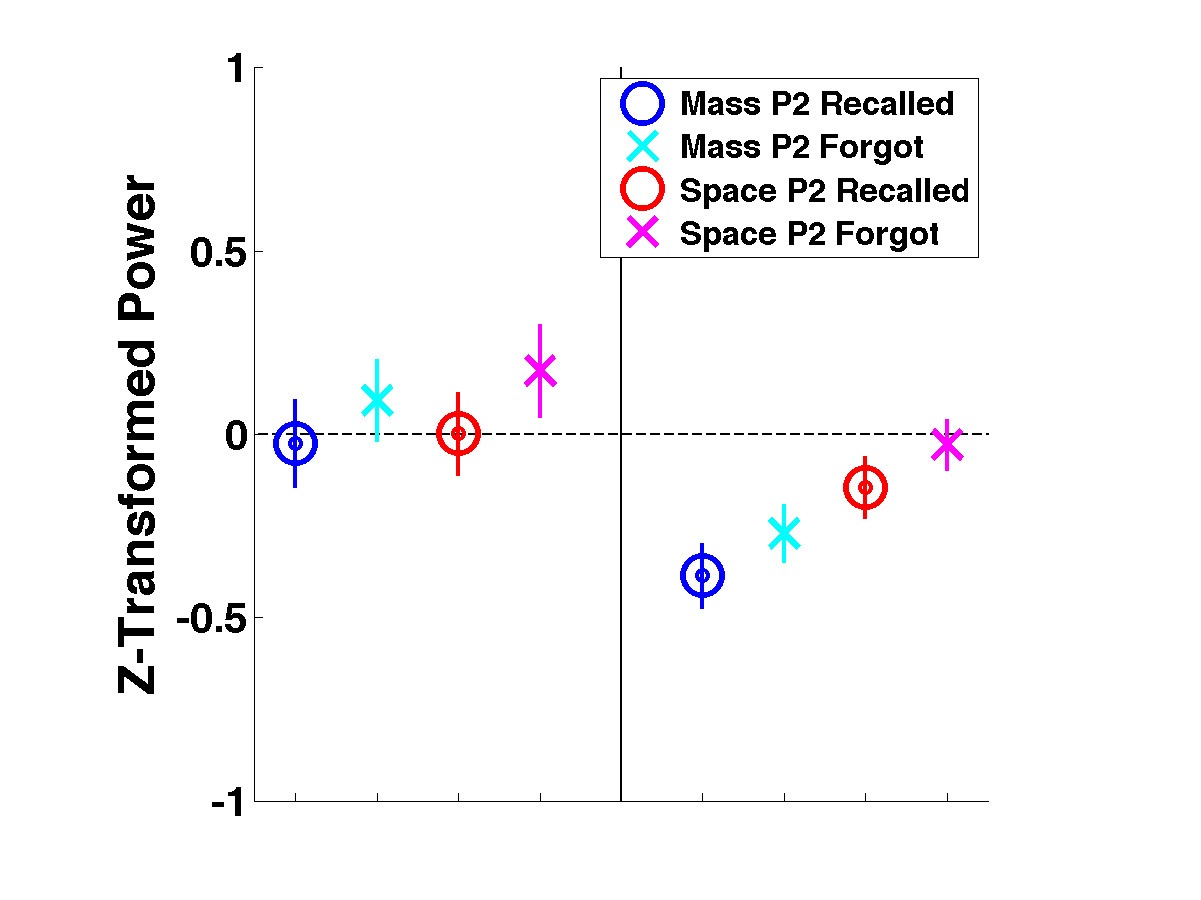
\includegraphics[width=.30\textwidth]{./figs/exp1/tfr_avg_ga_word_RgH_rc_mass_p2_word_RgH_fo_mass_p2_word_RgH_rc_spac_p2_word_RgH_fo_spac_p2_101ROI_0_500_500_1000_8_10_ylabel} \\
  & \multicolumn{1}{l}{(d)} & \multicolumn{1}{l}{(e)} & & \multicolumn{1}{l}{(f)} \\
  \raisebox{1.8cm}{\rotatebox{90}{Image}} & 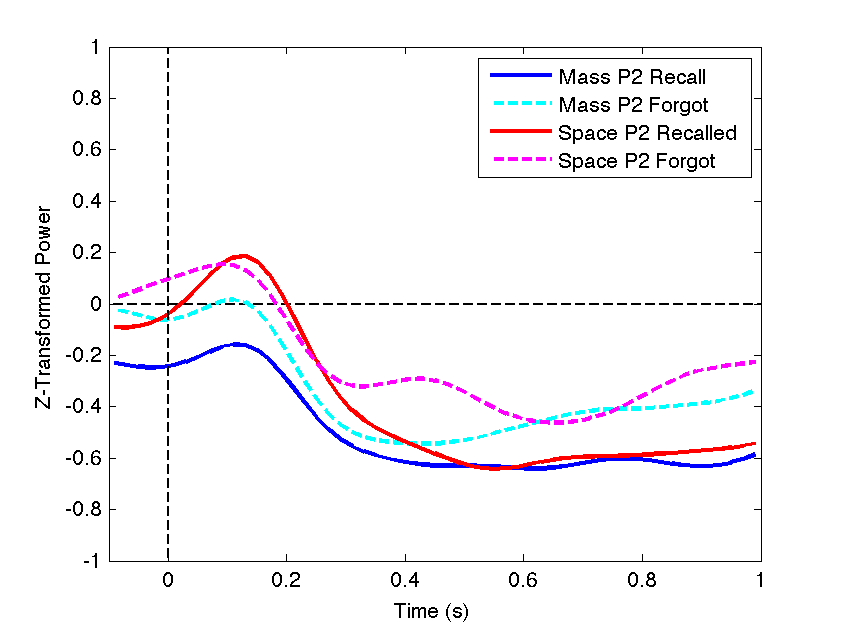
\includegraphics[width=.30\textwidth]{./figs/exp1/tfr_line_ga_img_RgH_rc_mass_p2_img_RgH_fo_mass_p2_img_RgH_rc_spac_p2_img_RgH_fo_spac_p2_89ROIs_-100_1000_8_10_legend} &
  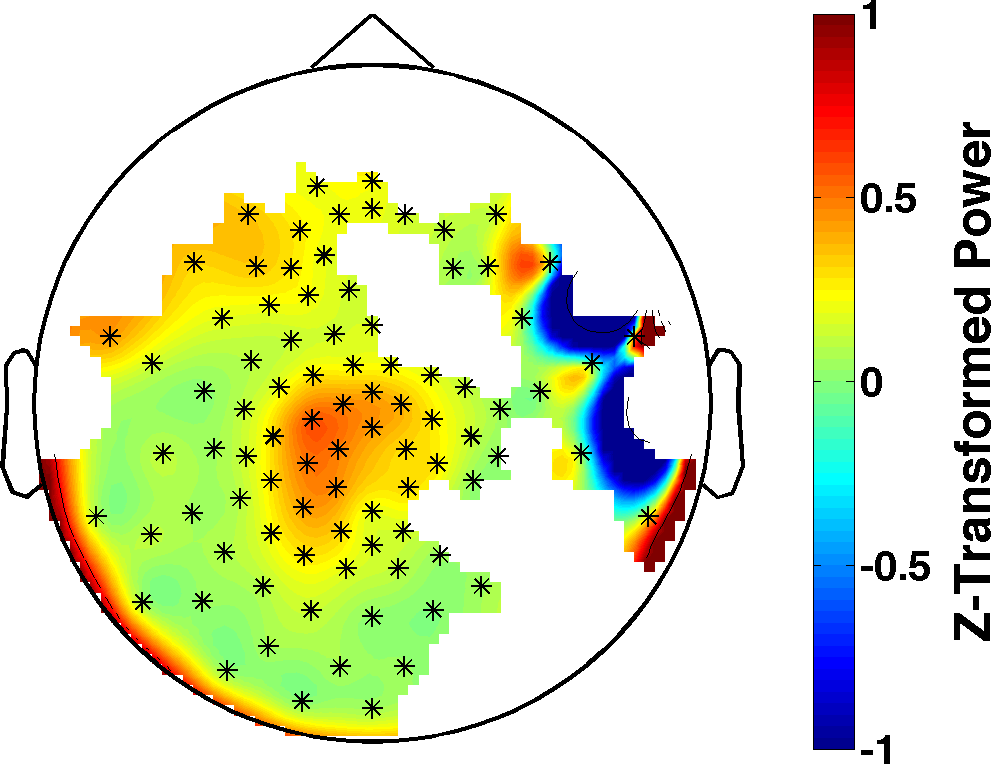
\includegraphics[width=.19\textwidth]{./figs/exp1/tfr_topocont_ga_img_RgH_rc_spac_p2vsimg_RgH_rc_mass_p2_89ROIs_8_10_0_500_-1p0_1p0_cb} &
  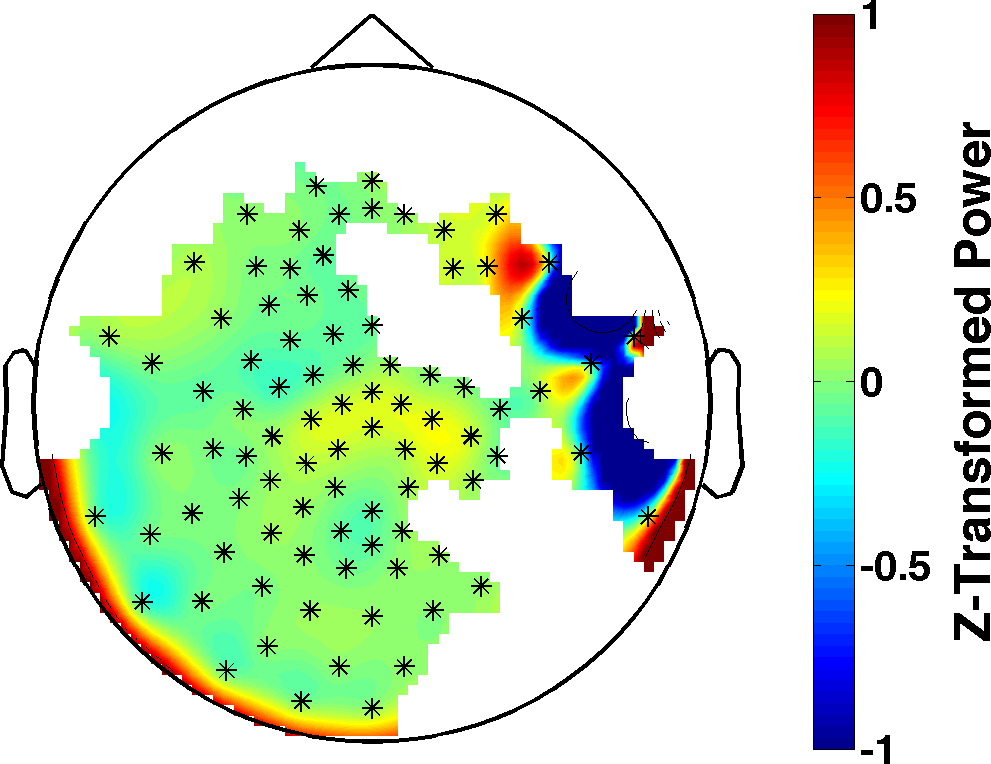
\includegraphics[width=.19\textwidth]{./figs/exp1/tfr_topocont_ga_img_RgH_rc_spac_p2vsimg_RgH_rc_mass_p2_89ROIs_8_10_520_1000_-1p0_1p0_cb} &
  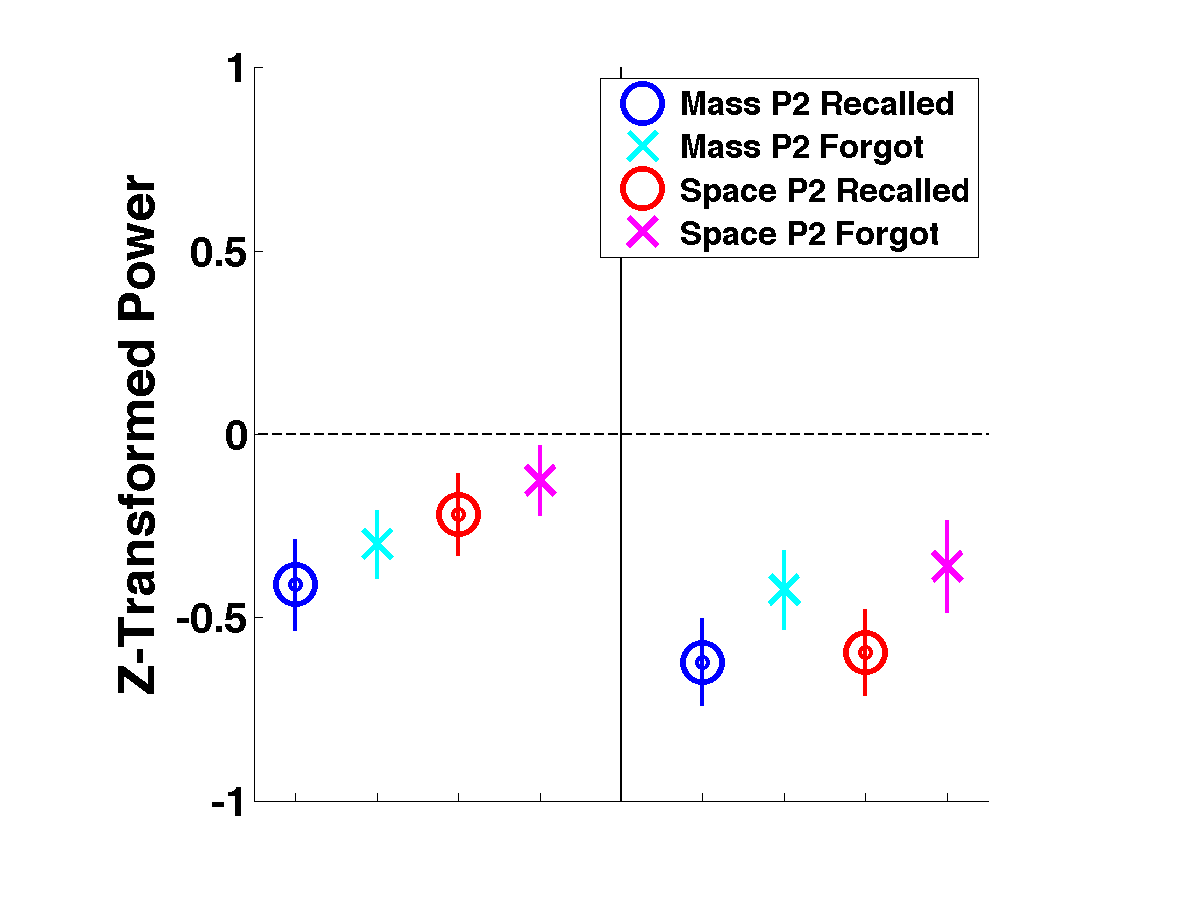
\includegraphics[width=.30\textwidth]{./figs/exp1/tfr_avg_ga_img_RgH_rc_mass_p2_img_RgH_fo_mass_p2_img_RgH_rc_spac_p2_img_RgH_fo_spac_p2_89ROI_0_500_500_1000_8_10_ylabel} \\
  \end{tabular}
  \caption{Lower alpha power to words and images.  (a) and (d) Grand averages; (b) and (e) contrast topographic plot between spaced and massed subsequently recalled trials displaying only the analyzed electrodes (*); (c) and (f) mean values for the two time windows (error bars are SEM).}
  \label{fig:word_img_alpha_low}
  %Figure~\ref{fig:word_img_alpha_low}
\end{figure}

\textit{Word, lower alpha}: Across 101 electrodes (Figure~\ref{fig:word_img_alpha_low}, top), lower alpha showed a spacing $\times$ time interaction [$F(1,22)=8.77, p=.0072$] such that massed words showed decreased alpha power compared to spaced in the second time window ($M=-0.323$ \textit{vs.} $M=-0.087$).
There were also main effects of spacing [$F(1,22)=7.64, p=.0113$] (massed showed less power), subsequent memory [$F(1,22)=5.4, p=.0298$] (recalled words showed less power), and time [$F(1,22)=15.3, p=.00074$] (less power in the later time window).

\textit{Image, lower alpha}: Across 89 electrodes (Figure~\ref{fig:word_img_alpha_low}, bottom), lower alpha for images showed the same results: a spacing $\times$ time interaction [$F(1,22)=5.19, p=.0329$] such that massed images had decreased power compared to spaced spaced in the first time window ($M=-0.352$ \textit{vs.} $M=-0.183$) but not the second ($M=-0.533$ \textit{vs.} $M=-0.497$).
There were also the same main effects of spacing [$F(1,22)=4.34, p=.0491$] (massed showed less power), subsequent memory [$F(1,22)=12, p=.0022$] (recalled words showed less power), and time [$F(1,22)=21.4, p=.000131$] (less power in the later time window).

% plot: word and image upper alpha
\begin{figure}[H]
  \centering
  \begin{tabular}{ccccc}
  & Upper alpha power & \multicolumn{2}{c}{Recalled P2: Spaced $-$ Massed} & Means \\
  &  & 0--500~ms & 500--1000~ms \\
  & \multicolumn{1}{l}{(a)} & \multicolumn{1}{l}{(b)} & & \multicolumn{1}{l}{(c)} \\
  \raisebox{1.8cm}{\rotatebox{90}{Word}} & 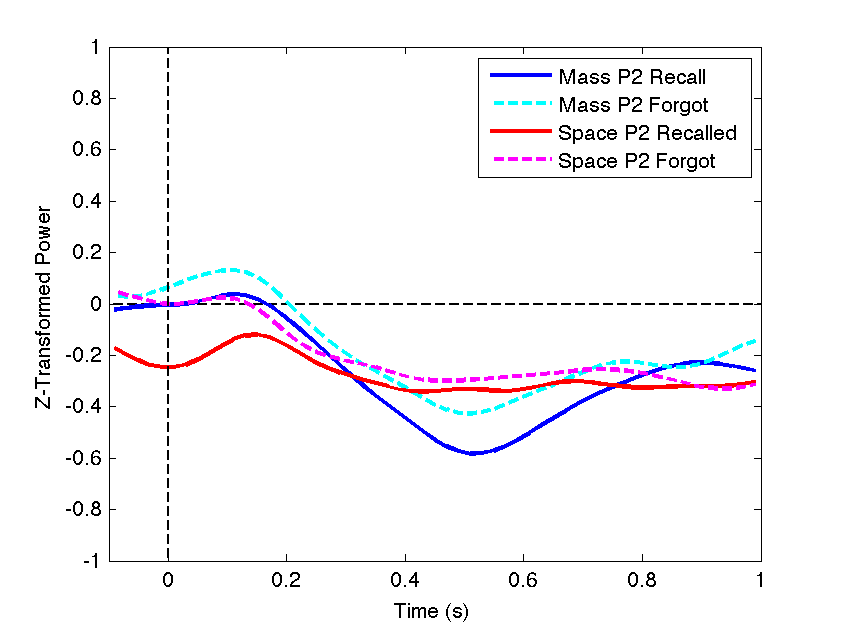
\includegraphics[width=.30\textwidth]{./figs/exp1/tfr_line_ga_word_RgH_rc_mass_p2_word_RgH_fo_mass_p2_word_RgH_rc_spac_p2_word_RgH_fo_spac_p2_82ROIs_-100_1000_11_12_legend} &
  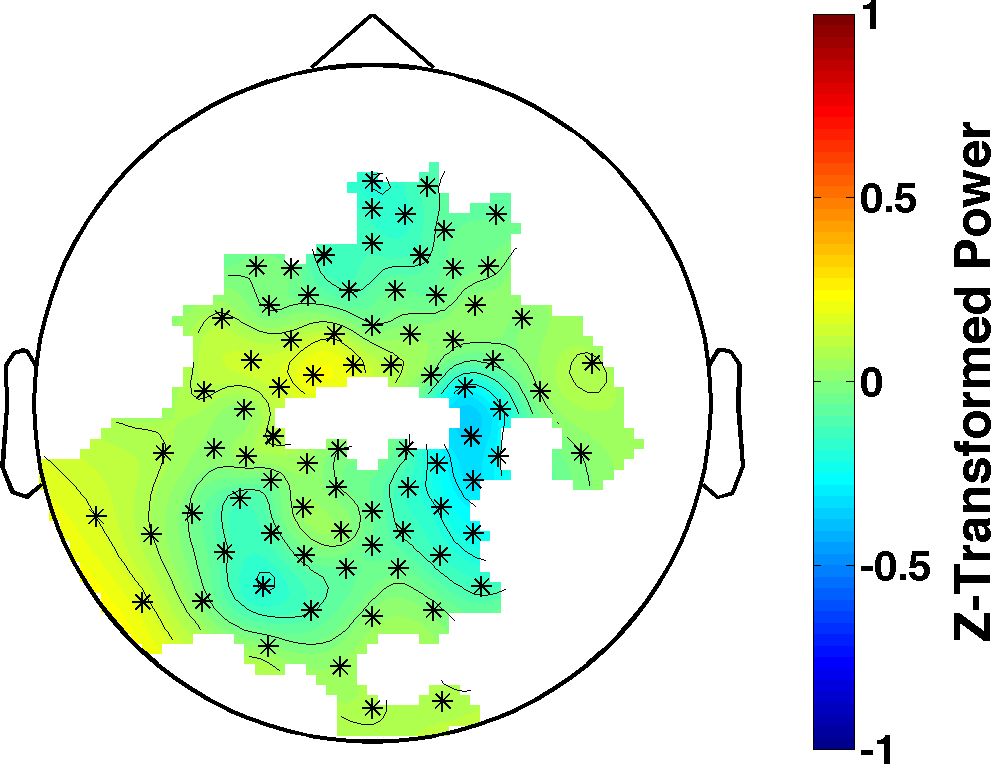
\includegraphics[width=.19\textwidth]{./figs/exp1/tfr_topocont_ga_word_RgH_rc_spac_p2vsword_RgH_rc_mass_p2_82ROIs_11_12_0_500_-1p0_1p0_cb} &
  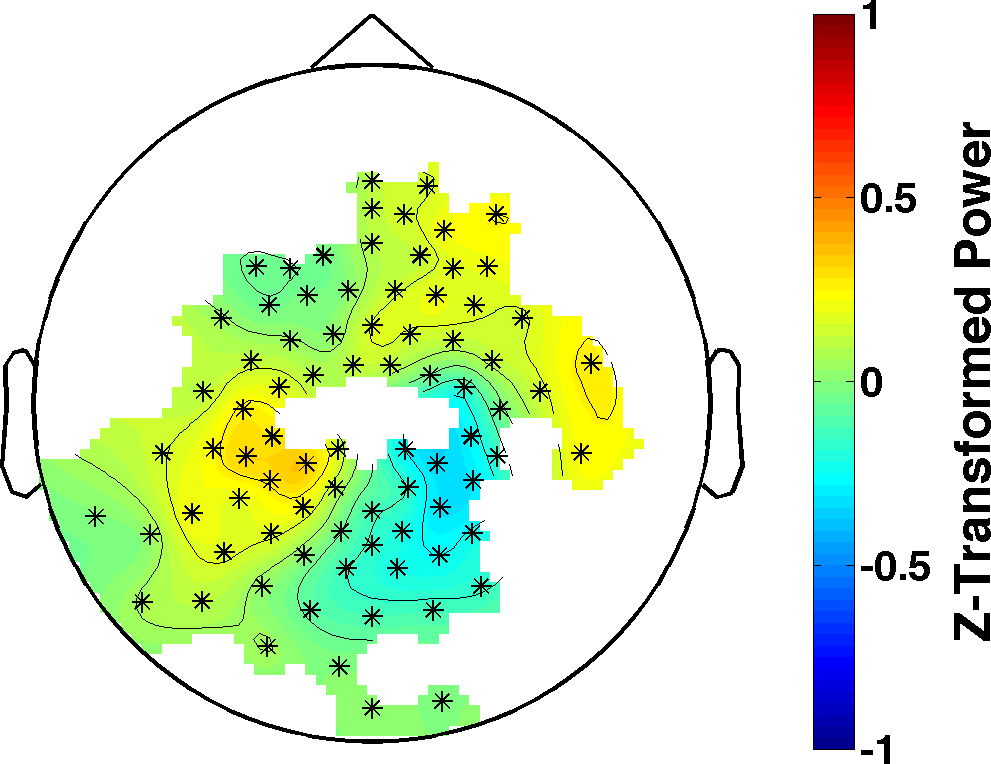
\includegraphics[width=.19\textwidth]{./figs/exp1/tfr_topocont_ga_word_RgH_rc_spac_p2vsword_RgH_rc_mass_p2_82ROIs_11_12_520_1000_-1p0_1p0_cb} &
  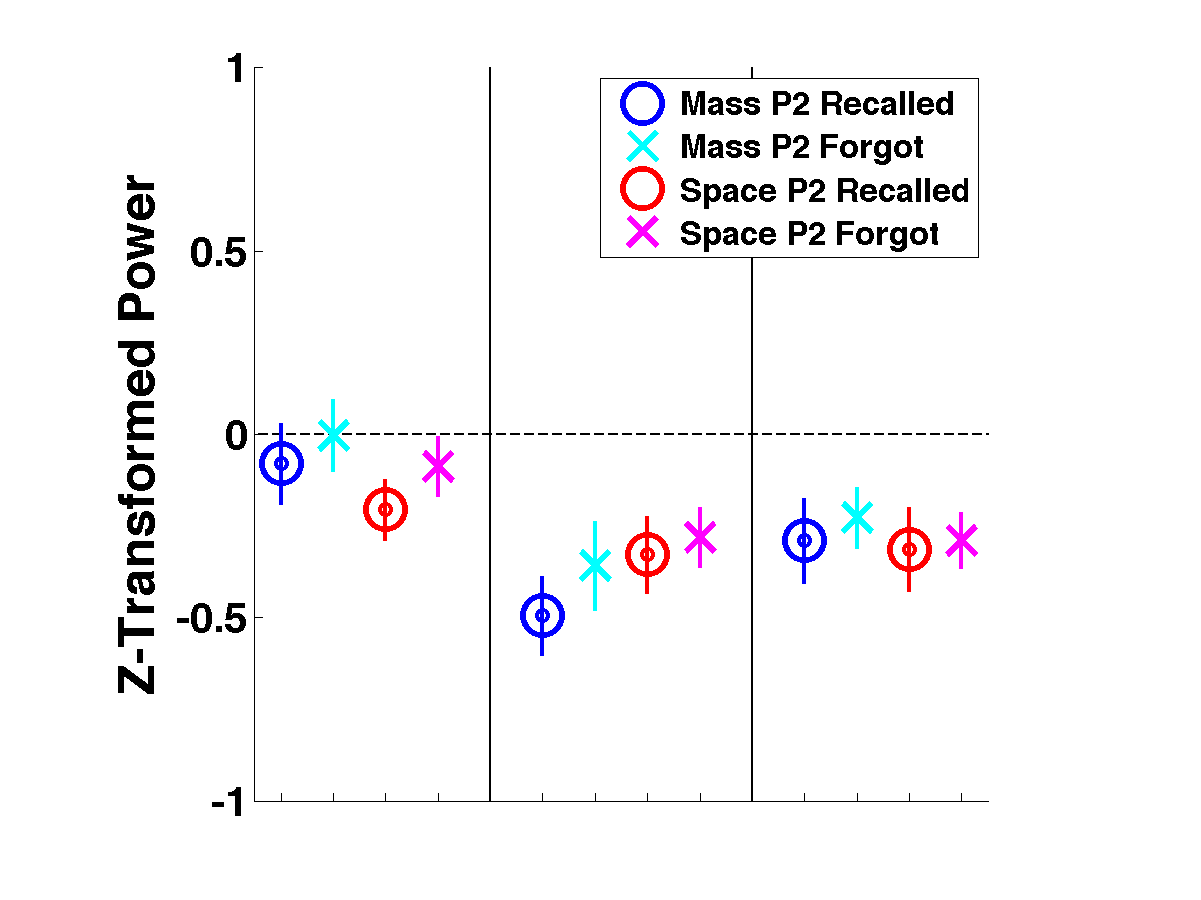
\includegraphics[width=.30\textwidth]{./figs/exp1/tfr_avg_ga_word_RgH_rc_mass_p2_word_RgH_fo_mass_p2_word_RgH_rc_spac_p2_word_RgH_fo_spac_p2_82ROI_0_333_333_666_666_1000_11_12_ylabel} \\
  & \multicolumn{1}{l}{(d)} & \multicolumn{1}{l}{(e)} & & \multicolumn{1}{l}{(f)} \\
  \raisebox{1.8cm}{\rotatebox{90}{Image}} & 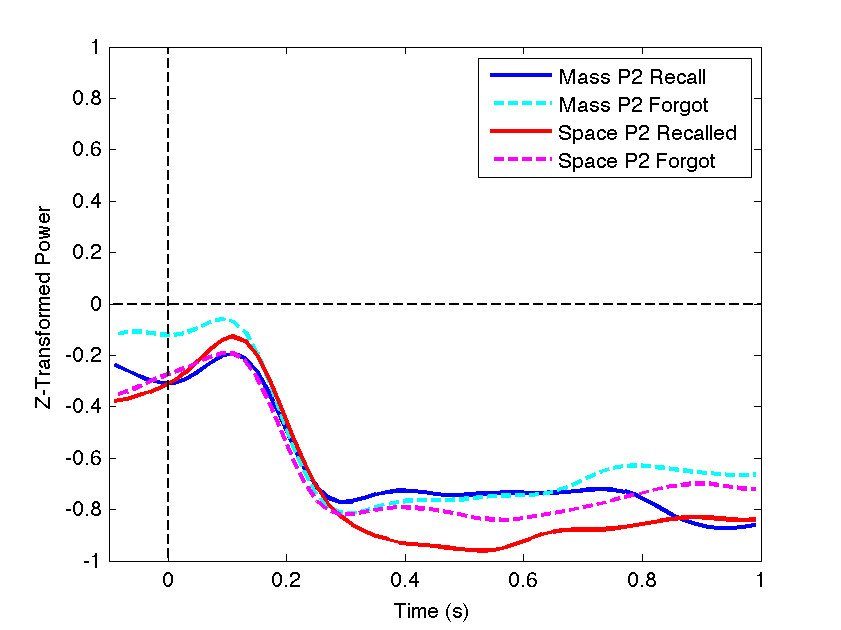
\includegraphics[width=.30\textwidth]{./figs/exp1/tfr_line_ga_img_RgH_rc_mass_p2_img_RgH_fo_mass_p2_img_RgH_rc_spac_p2_img_RgH_fo_spac_p2_30ROIs_-100_1000_11_12_legend} &
  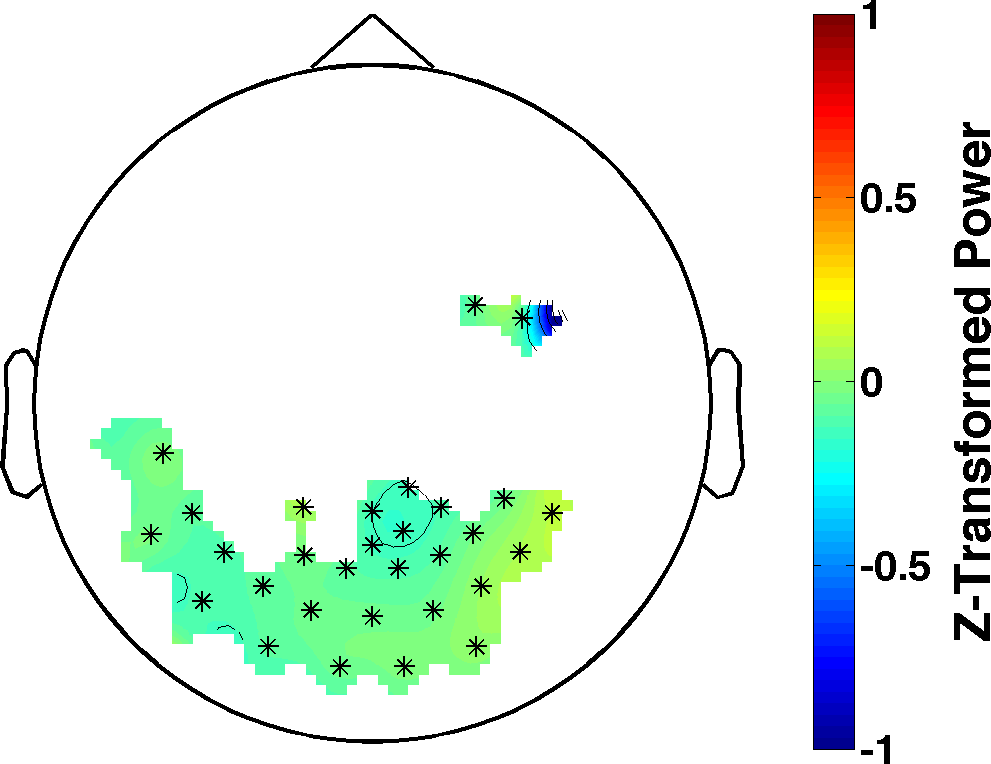
\includegraphics[width=.19\textwidth]{./figs/exp1/tfr_topocont_ga_img_RgH_rc_spac_p2vsimg_RgH_rc_mass_p2_30ROIs_11_12_0_500_-1p0_1p0_cb} &
  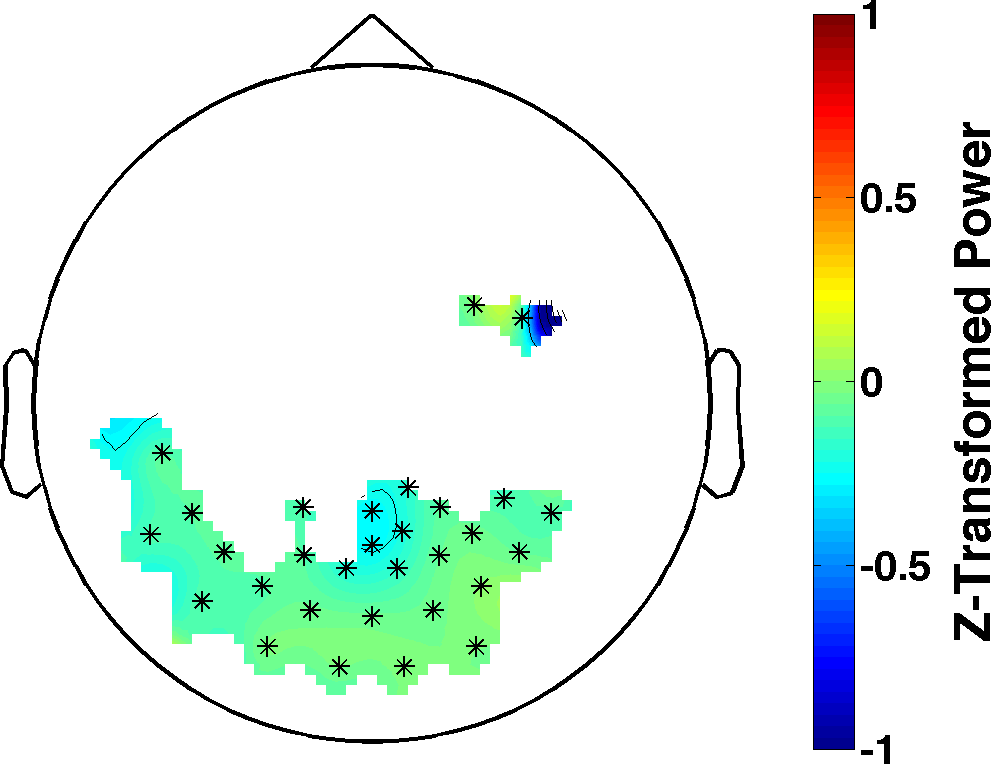
\includegraphics[width=.19\textwidth]{./figs/exp1/tfr_topocont_ga_img_RgH_rc_spac_p2vsimg_RgH_rc_mass_p2_30ROIs_11_12_520_1000_-1p0_1p0_cb} &
  \includegraphics[width=.30\textwidth]{./figs/exp1/tfr_avg_ga_img_RgH_rc_mass_p2_img_RgH_fo_mass_p2_img_RgH_rc_spac_p2_img_RgH_fo_spac_p2_30ROI_0_333_333_666_666_1000_11_12_ylabel} \\
  \end{tabular}
  \caption{Upper alpha power to words and images.  (a) and (d) Grand averages; (b) and (e) contrast topographic plot between spaced and massed subsequently recalled trials displaying only the analyzed electrodes (*); (c) and (f) mean values for the three time windows (error bars are SEM).}
  \label{fig:word_img_alpha_upp}
  %Figure~\ref{fig:word_img_alpha_upp}
\end{figure}

\textit{Word, upper alpha}: Across 82 electrodes (Figure~\ref{fig:word_img_alpha_upp}, top), upper alpha only showed a main effect of time for words [$F(1,22)=4.47, p=.0461$]; there was less power in the second time window than the first ($M=-0.309$ \textit{vs.} $M=-0.183$).  However, because the data clearly show a negative peak for recalled massed repetitions near 500~ms we divided time into three successive windows.  There was a robust spacing $\times$ time interaction [$F(2,44)=7.46, p=.00377$].  Massed were more negative in the middle time window than in neighboring time windows [$p$s~$<.05$], and were more negative than spaced in the first and second time windows [$p$s~$<.05$].

\textit{Image, upper alpha}: Across 30 electrodes (Figure~\ref{fig:word_img_alpha_upp}, bottom), upper alpha showed main effects of spacing [$F(1,22)=4.88, p=.0379$] (spaced had less power) and time [$F(1,22)=21.2, p=.000138$] (less power in the later time window).  Under the three time window ANOVA, there was also a significant three-way interaction [$F(2,44)=3.28, p=.05$]: recalled spaced repetitions in the middle time window were more negative than recalled massed repetitions in all time windows [$p$s~$<.005$], and recalled spaced repetitions in the late time window were more negative than the first two windows for massed [$p$s~$<.05$].  The same pattern was seen when comparing recalled spaced repetitions to forgotten massed repetitions [$p$s~$<.05$].  Additionally, recalled spaced repetitions were more negative in the middle time window and were more negative than forgotten spaced repetitions in the first and last time windows [$p$s~$<.05$].

% lower beta shows memory effects

% plot: word and image lower beta
\begin{figure}[H]
  \centering
  \begin{tabular}{ccccc}
  & Lower beta power & \multicolumn{2}{c}{Recalled P2: Spaced $-$ Massed} & Means \\
  &  & 0--500~ms & 500--1000~ms \\
  & \multicolumn{1}{l}{(a)} & \multicolumn{1}{l}{(b)} & & \multicolumn{1}{l}{(c)} \\
  \raisebox{1.8cm}{\rotatebox{90}{Word}} & \includegraphics[width=.30\textwidth]{./figs/exp1/tfr_line_ga_word_RgH_rc_mass_p2_word_RgH_fo_mass_p2_word_RgH_rc_spac_p2_word_RgH_fo_spac_p2_81ROIs_-100_1000_13_21_legend} &
  \includegraphics[width=.19\textwidth]{./figs/exp1/tfr_topocont_ga_word_RgH_rc_spac_p2vsword_RgH_rc_mass_p2_81ROIs_13_21_0_500_-1p0_1p0_cb} &
  \includegraphics[width=.19\textwidth]{./figs/exp1/tfr_topocont_ga_word_RgH_rc_spac_p2vsword_RgH_rc_mass_p2_81ROIs_13_21_520_1000_-1p0_1p0_cb} &
  \includegraphics[width=.30\textwidth]{./figs/exp1/tfr_avg_ga_word_RgH_rc_mass_p2_word_RgH_fo_mass_p2_word_RgH_rc_spac_p2_word_RgH_fo_spac_p2_81ROI_0_333_333_666_666_1000_13_21_ylabel} \\
  & \multicolumn{1}{l}{(d)} & \multicolumn{1}{l}{(e)} & & \multicolumn{1}{l}{(f)} \\
  \raisebox{1.8cm}{\rotatebox{90}{Image}} & \includegraphics[width=.30\textwidth]{./figs/exp1/tfr_line_ga_img_RgH_rc_mass_p2_img_RgH_fo_mass_p2_img_RgH_rc_spac_p2_img_RgH_fo_spac_p2_78ROIs_-100_1000_13_21_legend} &
  \includegraphics[width=.19\textwidth]{./figs/exp1/tfr_topocont_ga_img_RgH_rc_spac_p2vsimg_RgH_rc_mass_p2_78ROIs_13_21_0_500_-1p0_1p0_cb} &
  \includegraphics[width=.19\textwidth]{./figs/exp1/tfr_topocont_ga_img_RgH_rc_spac_p2vsimg_RgH_rc_mass_p2_78ROIs_13_21_520_1000_-1p0_1p0_cb} &
  \includegraphics[width=.30\textwidth]{./figs/exp1/tfr_avg_ga_img_RgH_rc_mass_p2_img_RgH_fo_mass_p2_img_RgH_rc_spac_p2_img_RgH_fo_spac_p2_78ROI_0_333_333_666_666_1000_13_21_ylabel} \\
  \end{tabular}
  \caption{Lower beta power to words and images.  (a) and (d) Grand averages; (b) and (e) contrast topographic plot between spaced and massed subsequently recalled trials displaying only the analyzed electrodes (*); (c) and (f) mean values for the three time windows (error bars are SEM).}
  \label{fig:word_img_beta_low}
  %Figure~\ref{fig:word_img_beta_low}
\end{figure}

\textit{Word, lower beta}:  Since lower beta oscillations showed a similar dip-and-rise pattern to upper alpha, we also used three time windows in these ANOVA.  Across 81 electrodes (Figure~\ref{fig:word_img_beta_low}, top), lower beta showed a spacing $\times$ time interaction [$F(2,44)=9.89, p=.000453$]; massed decreased most in the middle time window [$p<.01$] but spaced showed no differences across time.  There was also a marginal memory $\times$ time interaction [$F(2,44)=2.91, p=.0725$]; power for both recalled and forgotten stimuli was lowest in the middle time window [$p$s~$<.05$], but was most negative for recalled [$p<.01$].
A main effect of time [$F(2,44)=12.9, p=5.28e^{-5}$] and a marginal main effect of subsequent memory that followed the same patterns [$F(1,22)=4.16, p=.0536$].

\textit{Image, lower beta}: Across 78 electrodes (Figure~\ref{fig:word_img_beta_low}, bottom), lower beta showed main effects of memory [$F(1,22)=20.2, p=.00018$] (recalled had a power decrease) and time [$F(2,44)=29.3, p=1.14e^{-8}$] (less power in the middle time window).


\subsection{Time--frequency discussion}

Overall, there was higher theta power for spaced than massed repetitions during both words (late) and images (early).
% \hl{(AH asked: why difference in time for words and images?)}
Under study-phase retrieval, spaced repetitions will naturally require retrieval from long-term memory, thereby needing to engage processes related to episodic memory.  Since massed items are still primed and in working memory we would not expect these processes to engage.
Greater theta power for spaced repetitions than massed items denotes that recollection processes are engaged, and this supports study-phase retrieval.  Contextual variability does not require this retrieval, but both theories would posit that spaced items will be encoded (or re-encoded in the case of study-phase retrieval) with the evolved contextual state, and so theta should continue into the image presentation during processes that involve word--image binding (since participants were asked to link the stimuli).
\cbstart
Thus, it seems that associative retrieval engages during words and the re-encoding of word--image associations (binding) engages during images; this combination supports study-phase retrieval.  The negative SME for images, driven by massed items, is interesting.  Both positive and negative SMEs have been seen previously in the theta band.  \citeA{StauHans2013} actually changed the direction of the theta effect by varying context: same context showed a positive SME, different context showed a negative SME.  The present results only show a negative SME, though it seems unlikely that there are contextual difference for massed repetitions.
\hl{(Perhaps the remembered massed stimuli were encoded in a more variable fashion (e.g., thought about the stimuli in two different ways).)}
\cbend

% \citeA{KlimEtal2006} showed that early (200--400~ms) theta decreases as lag increases in a continuous recognition paradigm (shortest lag was 2 items; same pattern as the N400).  \citeA{VanSEtal2007} replicated this result for massed items (lag~$=0$).
% % Both of these studies had single-presentation items mixed in with repetitions.
% These previous results suggest that theta is related to memory trace strength in the short-term store (where strength decreases with lag).  However, we do not see this pattern of theta power.  Rather, it seems that our effects for spaced repetitions (more theta for words [late] and images [early]) are likely due to associative retrieval and the re-encoding of those associations (binding), respectively.  This is the more typical interpretation of theta in episodic memory research.  Somewhat surprisingly, theta power decreased during images and this showed a significant effect of subsequent recall (Figure~\ref{fig:word_img_theta}).  This seems driven by massed repetitions, but may be influenced by processes during the initial presentation.  Notably, recent work by \citeA{StauHans2013} found that theta showed a similar negative subsequent memory effect during a context mismatch condition (and a positive SME during context match); this leads to the possibility that memory performance for massed items increases when context is more variable, supporting the contextual variability theory for massed words only.

% Memory seems to show a clearer pattern in relation to attention and semantic processing (in alpha).

% Since our paradigm does not involve constantly testing oneself as continuous recognition does, our results seem more applicable to real-world learning.

The lower alpha band should correlate negatively with general attentional processes and should be widespread over the scalp.  Deficient processing would predict increased alpha power for massed repetitions.  We would also expect an effect of memory such that decreased power should be associated with better subsequent memory.
Lower alpha showed a sharp decrease during massed words that continued through images compared to spaced (going against the deficient processing prediction), as well as a main effect of memory.  This result indicates that more attention gets allocated to massed items and to subsequently recalled items overall.  In contrast to the visual N1 ERP component reported earlier, which is also related to attention, lower alpha does not show that massed repetitions are put at an attentional disadvantage; however, the timing difference between these effects implies that they are likely related to different mechanisms.
Nonetheless, lower alpha shows a different pattern from our deficient processing predictions.
\cbstart
Perhaps these effects follow the LPC and reflect attentional mechanisms accessing prior presentations of massed items more easily than spaced repetitions.
\cbend

Effects in the upper alpha band and lower beta band should occur late during the word and into the image presentation while semantic processes are engaged (associating the word and the image).  Because the semantic representation of massed items is still active, accessing this information may occur faster than for spaced items (like the LPC effect) but may not be processed as deeply.  We would also expect an effect of subsequent memory such that trials with more semantic processing (decreased power) are remembered better.  However, deficient processing would predict increased power, leading to decreased semantic processing of massed repetitions.

\cbstart
For upper alpha, we found a spacing $\times$ time interaction after dividing power for words into three time windows (massed word repetitions desynchronized sooner and to a greater extent than spaced). \cbend This supports the idea that semantic information for massed repetitions is accessed more quickly than for spaced.  Perhaps semantic information is quickly sought and retrieved for massed repetitions.  Upper alpha for words quickly returns to near-baseline levels (meaning it is inhibited because it no longer needs to be accessed) and spaced repetitions decreased in power (desynchronize) more during the image, supporting a deeper semantic processing of spaced word--image pairs overall.  Importantly, when considering three time windows for images the overall pattern in the three-way interaction showed that recalled spaced image repetitions were the most negative, denoting that increased semantic processing leads to better subsequent memory for spaced trials.

Lower beta showed power decreases for massed words (mostly driven by the recalled trials), and a general subsequent memory effect for images (power decrease is associated with better memory).  It seems that increased semantic processing (denoted by decreased power) helps memory overall, and massed trials get a quick semantic processing boost during word presentations but spaced are equally processed during the images.  Upper alpha and lower beta power decreases therefore seem to be related to processing semantic information after retrieval, with alpha showing an advantage for spaced and beta correlating more with overall subsequent memory performance.

\cbstart
Across this range of frequency bands, our results show that spaced repetitions involve (a) more retrieval and encoding (theta) starting in the latter half of the word presentation, possibly reflecting the retrieval and encoding of word--image associations, as well as (b) more semantic processing (upper alpha) for remembered spaced repetitions during the image presentation, possibly reflecting the semantic link being made between the word and image.
\cbend

% This seems in line with \citeA{Chal1993}?

% If massed repetitions are accessed more easily, why are spaced items (which by definition require retrieval from long-term memory) remembered better on average?  Is it simply due to the brain considering massed repetitions as more familiar and therefore devoting less processing to them?

% Remembered spaced repetitions show an increase in theta starting at about 600~ms during the word presentation, indicating that new information is being encoded.  It seems that because this spacing effect continues throughout the presentation of the paired image, item--context binding is occurring

% Overall the theta effect shows that in FS power remains high for spaced repetitions while it drops for massed repetitions, both regardless of subsequent memory. So where does the SME occur?  Perhaps it is not in the oscillations or ERPs but in the information that actually gets encoded (similarity analysis).

% Considering the upper alpha band, subsequently remembered massed repetitions induce desynchronization around the same time as lower alpha (500~ms).   at 800~ms remembered spaced repetitions desynchronize to a significantly greater extent than massed at central and right posterior sites, indicating semantic processing; this desynchronization continues through the image presentation.

% Upper alpha effect is the same as \citeA{VanSEtal2007}.

\subsection{Similarity results}

While the ERP and time--frequency results reveal that massed representations are accessed more quickly but perhaps to a lesser extent semantically than spaced representations, the nature of this representation is still unclear.  Are spaced repetitions remembered better due to essentially a repetition effect (in line with study-phase retrieval), or does temporocontextual drift play a role in encoding the repetition in a more variable manner (in line with contextual variability)?

EEG voltages during study image presentations were used to compute the neural similarity between each initial study presentation and its repetition.  This same process was done separately for time--frequency oscillations using the following bands: theta, alpha, lower beta, upper beta, lower gamma, upper gamma.  Images were used because this is when word--image binding
% (an item--context association)
should occur.  Neural similarity between study repetitions was assessed using the method from \citeA{MannEtal2011}.  All analyzed trials were subsequent hits (correctly recognized as being old), and were divided by the factors of spacing at study (spaced or massed) and subsequent recall at test (correctly recalled or not).
% Images were used because this is when an association would be made between the word--image pair.
The analyzed electrodes were influenced by the regions where \citeA{MannEtal2011} found context-related activity, but as this is a novel analysis the data were manually inspected and regions were chosen by hand (usually over occipital, temporal, and/or parietal regions).  Each trial was split into five 200~ms windows (processed and analyzed separately) under the idea that different cognitive mechanisms may occur at different points in time and that these mechanisms may affect the similarity measurement.

% Trials were further pared down by whether both image presentations could be correctly classified as showing neural activity for a face or a house.  An elastic net logistic regression classifier was trained on EEG for the exposure phase images to classify neural activity for faces and houses for the same electrodes and samples, and was then tested on each study presentation.  The L1/L2 mixing parameter ($\alpha$) was set to $0.2$; the shrinkage parameter ($\lambda$) was determined by cross validation.  This allows us to find the trials for which there is image-related ``signal'' in the EEG (however, this method may actually have theoretical issues, discussed below).

% 20 participants who had three or more correctly classified trials were included in the analysis.

Principal Components Analysis (PCA) was used for dimensionality reduction; for each subject, a three-dimensional matrix of voltage measurements (trials by electrodes by time samples) was reshaped into a two-dimensional matrix by unrolling electrodes and time within a trial.  Similarly, a matrix with the additional dimension of frequency band was used when analyzing these data.  For each time window, PCA was run on this two-dimensional matrix and the Kaiser criterion was used to choose the components that explained a substantial portion of the variance (eigenvalues~$>1$; \citeNP{Kais1960}).
%components that explained 85\% of the variance were retained.
Each retained component is a linear combination of the neural activity (voltage or power for each frequency band) across electrodes and time samples.  Each trial then has a weight from each principal component, and together these weights yield the trial's feature vector.  The similarity measurement is computed using the normalized dot product of a given item's repetitions (the cosine of the angle between the feature vectors).  Finally, the between-trial similarity values for each participant (comparing each event with every other analyzed event, not just its repetition pair) are z-scored so they are in standard deviation units.  Thus, a similarity value of zero means the representation is of average similarity compared to all events, and a positive or negative deviation from there means similarity increases or decreases relative to all events.

% Before z-scoring, a dot product of 1 would mean the representation are identical (the feature vectors overlap), a dot product of -1 would mean the representations are completely dissimilar (the feature vectors are diametrically opposed), a dot product of zero means the representations are independent (the feature vectors are orthogonal.


% Perhaps there is a way to select principal components that vary with memory performance and/or encoding strength.

A three-way repeated measures ANOVA was run on the average voltage similarity values from left and right temporal regions with factors of spacing (spaced and massed), subsequent memory (recalled and not recalled), and time (successive time bins).  A main effect of spacing was found [$F(1,27)=29.8, p=8.91e^{-6}$] such that spaced presentations ($M=0.0777$) were more similar than massed ($M=-0.0886$), and a main effect of time was found [$F(4,108)=6.76, p=8.68e^{-5}$] such that neural similarity decreased over time.
This latter effect is explained by an interaction between spacing and time [$F(4,108)=9.58, p=2.36e^{-6}$].  Here, spaced items kept a relatively consistent level of similarity across the time windows whereas massed items become dramatically dissimilar as time progressed.  The three-way interaction was not significant [$F(4,108)=1.18, p=.323$] but the data are plotted in Figure~\ref{fig:sim_tla_spacXmemXtime}.


% thus, massed 500--1000~ms window shows significantly less similarity than that of spaced and the early spaced and massed windows.
% There was no interaction between spacing and subsequent memory [$p=.31$], but as would be expected from the main effect of spacing, spaced items were more similar than massed for both recalled and forgotten.

% \begin{figure}
%   \centering
%   \includegraphics[width=.40\textwidth]{./figs/exp1/similarity_spacXmem_tla_LPI2LPSLTRPI2RPSRT_0to500_500to1000_kaiser_cosine}
%   \caption{Similarity: Marginal interaction between spacing and subsequent memory.  Large symbols are grand averages, small symbols are individual participant averages.}
%   \label{fig:similarity_spacXsm}
%   %Figure~\ref{fig:similarity_spacXsm}
% \end{figure}

\begin{figure}
  \centering
  %\includegraphics[width=.40\textwidth]{./figs/exp1/similarity_spacXmemXtime_img_tla_LTRT_0to500_500to1000_kaiser_cosine}
  \includegraphics[width=.40\textwidth]{./figs/exp1/similarity_spacXmemXtime_img_tla_LTRT_0to200_200to400_400to600_600to800_800to1000_kaiser_cosine}
  \caption{Similarity for voltage at left and right temporal sites during image repetitions: Interaction between spacing, memory, and time [$n.s.$].}
  \label{fig:sim_tla_spacXmemXtime}
  %Figure~\ref{fig:sim_tla_spacXmemXtime}
\end{figure}


The same three-way ANOVA was performed for time--frequency data over left and right parietal regions across all frequency bands.  A significant effect of spacing was found [$F(1,27)=7.44, p=.0111$], but in the opposite direction of the voltage results: massed ($M=0.318$) were more similar than spaced ($M=0.243$).  There was also a main effect of time [$F(4,108)=3.42, p=.0116$], which was driven by an interaction with subsequent memory [$F(4,108)=6.3, p=.000206$] such that recalled images showed an increase in similarity at the last time window ($M=0.37$) compared to forgotten images ($M=0.26$) [$t(27)=2.7614, p=.0102$].
Finally, the three-way interaction was marginal [$F(4,108)=2.42, p=.0535$] and is plotted in Figure~\ref{fig:sim_pow_spacXmemXtime}.  The pattern shows that remembered items tend to increase in similarity in the second half of the trial while forgotten items tend to decrease; this increase is steeper for spaced compared to massed, though massed seem to receive a similarity boost earlier.

\begin{figure}
  \centering
  %\includegraphics[width=.40\textwidth]{./figs/exp1/similarity_spacXmemXtime_img_pow_PS_0to500_500to1000_kaiser_cosine}
  \includegraphics[width=.40\textwidth]{./figs/exp1/similarity_spacXmemXtime_img_pow_LPSRPS_0to200_200to400_400to600_600to800_800to1000_kaiser_cosine}
  \caption{Similarity for oscillatory power at left and right parietal sites during image repetitions: Interaction between spacing, memory, and time [$p=.0535$].}
  \label{fig:sim_pow_spacXmemXtime}
  %Figure~\ref{fig:sim_pow_spacXmemXtime}
\end{figure}

\subsection{Similarity discussion}

% Based on measurements of neural similarity.
It is clear that the way massed and spaced stimuli are processed and represented across their repetitions is different.  Surprisingly, the patterns are different for voltage and time--frequency data.  It is difficulty to know exactly what a decrease in similarity means; perhaps it indicates a decrease in processing, or perhaps it indicates more variable processing.  For voltage, it seems that spaced repetitions tend to induce a consistent representation across time, \cbstart which might support the study-phase retrieval account in that the same representation is being recalled and re-encoded across the trial. \cbend  Massed repetitions become much more variable either because noise is added to the system (a possible explanation supporting deficient processing), they tend to induce a more variable representation (supporting contextual variability), or different neural/cognitive processes are engaged.
The early attentional ERP results would seem to corroborate support for the deficient processing hypothesis, but only if ERPs to words affect processing of the rest of the trial (including images).
% but one would think that there would have been an effect of memory within massed trials (those massed item that were not deficiently processed would, on average, be subsequently remembered). \hl{(corroborate for words, but these are for images.)}

For the time--frequency analysis, the increase in similarity leading to the subsequent memory effects supports study-phase retrieval (or the engagement of the same processes) for both massed and spaced repetitions, especially toward the end of the trial.  No other spacing effect accounts seem to be supported with this analysis.

% TODO
%This is only a first pass and this method needs to be improved; two options are (a) to limit the principal components to those that are meaningful for a specific analysis as in \citeA{MannEtal2011} (e.g., keep those that show a correlation with memory), and (b) to utilize other comparisons of neural similarity such as the toolbox used by \citeA{SuEtal2012} that includes spatiotemporal searchlight functions\footnote{I have been in contact with the lead author and acquired their toolbox, but the package is complicated and I have not yet successfully used it.}.



% Perhaps it is the case that cued recall relies more on associative strength and less on context \cite[p.~107]{DelaEtal2010}.

% \subsection{Electrophysiological results: Classification}

% Attempt to classify image-related activity during the word repetition.

\section{Experiment~1 Discussion}

Behaviorally, participants showed a clear spacing effect for both recognition and recall, even using relatively short lags (compared to real-world learning).

It seems possible that memory effects might be relatively weak because subsequent memory only contrasted recalled \textit{vs.} forgotten.  Because every trial was a recognition hit, we can assume that at least the images were encoded at a reasonable level, since these are the stimuli shown at the recognition prompt.  It would be ideal to analyze the data for recognition miss trials, but accuracy was so good that there are very few miss trials.

\cbstart
Neural activity related to subsequent memory for spaced and massed repetitions is a critical factor to analyze in relation to the spacing effect.  The three-way interactions between spacing, repetition, and memory were significant for N1 voltage and upper alpha power, and marginal for time--frequency similarity.  Overall, this leads to the idea that increased attention for spaced items (as indexed by the N1) and semantic processing during word--image binding for spaced items (as indexed by upper alpha) benefits subsequent memory.
%The nature of neural representations across repeated study episodes should be explored further.
Integration across the neural effects is discussed below.  \hl{(TODO: Delete the last sentence and integrate these paragraphs more naturally.)}


Early attentional mechanisms orient more to spaced repetitions than massed (N1 more negative for spaced), especially for those that are subsequently recalled.  The N1 may be a signal to the system for when stimuli should receive additional processing (related to the N400 and upper alpha).  In fact, using source localization, \citeA{ProvAdor2009} found that the N170 has neural generators in regions that support semantic processing (BA10).  This N1 difference supports deficient processing.


A more negative N400 has been found to correlate with both semantic processing and subsequent memory, though there is not always a memory effect \cite<reviewed in>{FrieJohn2000}.  We simply found that voltage was more negative for spaced repetitions compared to massed, and was most negative for initial presentations.  This reflects that semantic processing decreases for massed repetitions, and also supports deficient processing.  The main effect of memory for the N400 shows that subsequent memory is better when semantic processing is engaged to a greater extent during encoding.  Matching these results overall, upper alpha showed the important interaction with memory such that remembered spaced repetitions had the largest power decrease.  This is another sign that there is more semantic processing for remembered spaced items.

Our results support the idea that massed representations are accessed more quickly and to a greater extent on repetition trials than for spaced repetitions (LPC more positive for massed).  Here, massed items are easily accessible because they are still in working memory, whereas spaced items need to be retrieved from long-term memory; this latter point is evident in the theta spacing main effect and interactions with time.  However, because massed repetitions feel more familiar due to having greater memory strength, it seems that they are not subjected to additional semantic processing, as mentioned above.
% Matching these effects, increased theta power for spaced compared to massed repetitions reflects that retrieval occurred (word, late) and encoding/binding is engaged (image, early).

\cbstart
In relation to the neural similarity of massed and spaced presentations (Figure~\ref{fig:sim_tla_spacXmemXtime}), massed items decreased in similarity while spaced items maintained a consistent amount.  Contextual variability predicts that context has not drifted between massed presentations, but this is not the effect we see.  Deficient processing does predict this decrease in similarity.  Another possibility for this pattern of results is the differential activation of neural processes across repetitions (e.g., the same noun is interpreted two different ways), but combined with the attention (N1) and semantic processing (N400) results, deficient processing seems more likely.  For spaced items maintaining similar neural patterns, either the same memory representation is retrieved at the second presentations, the same processes are engaged, or both of these occur.  This can support study-phase retrieval, and deeply challenges contextual variability.
\cbend

The combination of effects for spaced repetitions, from word--image binding (theta oscillation effects) to stable voltage similarity to increased power similarity, seems to support study-phase retrieval for these items that need to be retrieved from long-term memory, and does not yield support for contextual variability.  This is because increased theta has been associated with increased episodic retrieval.  Massed items, on the other hand, tend to be more variable; these EEG effects seem more in line with deficient processing than contextual variability.
% especially because the concept of temporocontextual drift (which meshes well with contextual variability) would likely predict almost no drift at massed repetitions.

\cbend
